%% 
%% Copyright 2007-2025 Elsevier Ltd
%% 
%% Knowledge-Based Systems - NeuroSLAM Paper
%% 

\documentclass[review,12pt]{elsarticle}
\journal{Knowledge-Based Systems}

\usepackage{booktabs}
\usepackage{tabularx}
\usepackage{ragged2e}
\usepackage{amsmath,amssymb,amsfonts}
% \usepackage{algorithmic}   % no algorithm environment in the body; switch to algorithm2e if the journal requires it
% \usepackage{algorithm}
\usepackage{array}
\usepackage[caption=false,font=normalsize,labelfont=sf,textfont=sf]{subfig}
\usepackage{url}
\usepackage{xurl}
\emergencystretch=1.5em
% float alignment: top-align full-page floats to remove the large vertical gaps of centred full-page figures
\makeatletter
\setlength{\@fptop}{0pt}
\makeatother
% float parameters: large figures prefer top-of-page floats, body text fills the space below, full-page floats must occupy 80% of the page height
\renewcommand{\topfraction}{0.9}
\renewcommand{\dbltopfraction}{0.9}
\renewcommand{\textfraction}{0.05}
\renewcommand{\floatpagefraction}{0.8}
\renewcommand{\dblfloatpagefraction}{0.8}
\usepackage{graphicx}
% graphics path (points to the local fig/ directory)
\graphicspath{{fig/}}
\usepackage{xcolor}
\usepackage{multirow}
\usepackage{threeparttable}
\usepackage[expansion=false]{microtype}
\usepackage{xspace}
\usepackage{lineno}

% line numbers (required in review mode)
\modulolinenumbers[5]

% custom colours (drawing only)
\definecolor{darkgreen}{rgb}{0,0.6,0}

\DeclareMathOperator*{\argmin}{\arg\!\min}
\DeclareMathOperator{\clip}{clip}
\DeclareMathOperator{\wrap}{wrap}

% Abbreviation macros
\makeatletter
\DeclareRobustCommand\onedot{\futurelet\@let@token\@onedot}
\def\@onedot{\ifx\@let@token.\else.\null\fi\xspace}

\def\eg{\emph{e.g}\onedot} \def\Eg{\emph{E.g}\onedot}
\def\ie{\emph{i.e}\onedot} \def\Ie{\emph{I.e}\onedot}
\def\cf{\emph{c.f}\onedot} \def\Cf{\emph{C.f}\onedot}
\def\etc{\emph{etc}\onedot} \def\vs{\emph{vs}\onedot}
\def\wrt{w.r.t\onedot} \def\dof{d.o.f\onedot}
\def\etal{\emph{et al}\onedot}
\makeatother


% title and authors (elsarticle frontmatter: after \begin{document}, before the body)
\begin{document}

\begin{frontmatter}

\title{Brain-Inspired 4-DoF Localization-Mapping with Hippocampal--Entorhinal Spatial Representations}

% corresponding e-mail (HUTB domain, hutb.edu.cn)
\author[hutb,xjl]{Haidong Wang\corref{cor1}}
\ead{open@hutb.edu.cn}
\author[hutb]{Rongbo Yang}
\ead{825404295@qq.com}
\author[hutb]{Caixia Ning}
\ead{ningcaixia064@gmail.com}
\author[hutb]{Yang Gao}
\ead{1723196099@qq.com}
\author[hutb]{Xiangyu Liu}
\ead{2437318001@qq.com}
\cortext[cor1]{Corresponding author.}

\affiliation[hutb]{organization={School of Artificial Intelligence and Robotics, Hunan University of Technology and Business},
            city={Changsha},
            postcode={410205},
            country={China}}
\affiliation[xjl]{organization={Xiangjiang Laboratory},
            city={Changsha},
            postcode={410205},
            country={China}}

\begin{abstract}
    \sloppy
    Monocular visual-inertial odometry recovers the shape of a trajectory but not its metric scale: the estimate is defined only up to a similarity transform, so scale error propagates into every downstream quantity, and drift can be removed only where the vehicle recognises ground it has already mapped. This paper presents NeuroLocMap, a brain-inspired localization-mapping framework formulated in a four-degree-of-freedom (4-DoF) state that couples vestibular--visual complementary fusion with hippocampal--entorhinal spatial representations. The pipeline combines dual-stream visual processing for appearance and motion, inertial integration, a three-dimensional grid-cell attractor for position encoding and an experience map for loop closure, all built on a fixed-dimension 10-state EKF core; two train-once components are attached downstream of the filter, a scale-only monocular correction over a frozen depth model and an embedding-based loop-closure channel. Across five scenarios, four CARLA towns (Town05/03/07/10HD) and one real highway sequence (KITTI~07), the full system reduces error against the 10-state EKF visual-inertial baseline on every scenario under both evaluation calibers, including 1.5--33.9\% under the rigid SE(3) caliber, where an incorrect metric scale cannot be absorbed by the alignment. On a closed-loop benchmark the experience-map re-anchoring reduces terminal displacement from 842.54~m to 55.92~m. The reference implementation runs in real time on a CPU, and its learned components transfer from simulation without per-domain retraining.
\end{abstract}

\begin{keyword}
Brain-inspired localization-mapping \sep Vestibular-visual fusion \sep Hippocampal--entorhinal spatial cells \sep Grid cells \sep Visual place recognition \sep Cognitive mapping
\end{keyword}

\end{frontmatter}

%% ==================== INTRODUCTION ====================
\section{Introduction}
\label{sec:intro}

Localization and mapping in three-dimensional environments underpins autonomous driving, mobile robotics and intelligent transportation systems~\cite{cadena2016past}. Practical systems combine cameras, inertial measurement units and, where available, satellite positioning to obtain a pose estimate, and the estimate itself is almost always produced by an optimiser or a filter~\cite{saputra2018visual}. Two costs follow from that choice. The first is transparency: the map is an artefact of the solver, and the quantities that produced it, feature tracks and marginal covariances, carry no spatial meaning that a human or a planner can read. The second is computation: where visual features enter the state, the per-update cost grows with their number, which is the customary obstacle to deployment on embedded hardware.

Biological navigation pays neither cost. Bats localise in three dimensions by combining visual and vestibular signals with spatially selective cells of the hippocampal formation~\cite{jeffery2013navigating,hafting2005microstructure,taube1990head,finkelstein2016three,solstad2008representation}. The circuits involved, grid cells, head-direction cells and place cells, hold position and orientation in a representation that is at once metric, low-dimensional and readable as a map. The appeal of this architecture for robotics is therefore not metaphorical: it suggests a state whose dimension is fixed by the encoding rather than by scene complexity.

Transferring the principle to a working system meets three difficulties. Most existing bio-inspired frameworks are planar, whereas road and indoor deployment requires a three-dimensional representation together with heading. Their visual front-ends rest on intensity templates whose discrimination degrades under illumination and viewpoint change, so place recognition fails where it is most needed. And fusion, where present, is either ad hoc or borrowed from tightly coupled optimisation, which reintroduces the feature-dependent cost that the biological architecture avoids.

This paper presents NeuroLocMap, a brain-inspired localization-mapping framework formulated in the 4-DoF pose $(x,y,z,\psi)$: a dual-stream visual front-end separates appearance from motion (ventral for scene recognition, dorsal for motion extraction), a vestibular front-end processes inertial data, and the two are combined by a frequency-domain fusion core that instantiates complementary filtering as a fixed-dimension (10-state) EKF. Position is encoded by three-dimensional grid cells, heading by multilayered head-direction cells, and place by a multilayer experience map that serves as an episodic memory for recognition and drift correction. The restriction to four degrees of freedom is deliberate. On road and indoor surfaces the orientation is dominated by yaw, while pitch and roll stay within the range imposed by vehicle dynamics (below $5^\circ$), so a 4-DoF state captures the motion that matters at a fraction of the state dimension of a full pose graph~\cite{milford2004ratslam,milford2010persistent}.

The contributions of this paper are as follows.
\begin{itemize}
    \item \emph{Architecture.} Dual-stream visual processing, vestibular modelling and hippocampal--entorhinal spatial representations are coupled into a single 4-DoF pipeline, with the filter, the spatial cells and the experience map operating on one state rather than as stacked modules.
    \item \emph{Visual front-end.} An explicit template-creation operator replaces the fixed template set of RatSLAM; across the evaluated sequences the template count rises from 5 to 964, and it is this increase that sustains place discrimination under illumination and viewpoint change.
    \item \emph{Fusion core.} A fixed-dimension 10-state EKF applies its gated branches in a fixed order, so per-update cost is independent of feature count; two train-once corrections, a scale-only depth-model head and an embedding-based loop-closure line, act downstream and never write back.
    \item \emph{Evaluation.} On four CARLA towns and KITTI~07 the system reduces error against the EKF baseline on all five scenarios under the rigid SE(3) caliber, where an unrecovered scale cannot be absorbed, and cuts closed-loop terminal displacement from 842.54~m to 55.92~m; the resulting experience graph is inspectable by construction.
\end{itemize}

In knowledge-based terms, the experience map produced by our pipeline serves as an explicit and interpretable topological knowledge representation, and loop closure operates as retrieval over this representation together with consistency-based correction of it.

%% ==================== RELATED WORK ====================
%% ==================== RELATED WORK ====================
\section{Related Work}
\label{sec:related}

Three literatures bear on this work: visual-inertial SLAM, which supplies the tracking core; brain-inspired spatial cognition, which supplies the state representation; and learning-based visual processing, which supplies much of the front-end. Each is summarised below with an explicit statement of where NeuroLocMap departs from it, and Table~\ref{tab:comparison_bioslam} collects the architectural differences.

\subsection{Visual SLAM and Sensor Fusion}
\label{sec:related_slam}

Visual SLAM has developed along two lines. Feature-based systems such as ORB-SLAM~\cite{mur2015orb} extract sparse keypoints and reach real-time performance in textured scenes; direct systems such as LSD-SLAM~\cite{engel2014lsd} and DSO~\cite{engel2018direct} operate on pixel intensities without feature extraction and recover semi-dense structure. Place recognition and loop closure have their own tradition, from the probabilistic bag-of-words model of FAB-MAP~\cite{Cummins2008} to the learned descriptors of NetVLAD~\cite{Arandjelovic2016}, with recent work pushing learned descriptors toward parameter-efficient transfer across seasons and sensors~\cite{wu2026pevpr}. Two constraints recur across this literature. Feature-based pipelines require texture, typically hundreds of keypoints per frame, and degrade in its absence; direct pipelines require photometric stability and tolerate neither motion blur nor uncalibrated exposure. In both cases the dominant cost is attached to the visual measurements themselves, whether through extraction and matching or through dense photometric optimisation.

Fusing an IMU with the camera removes part of that dependence, since inertial data is unaffected by illumination and supplies the high-frequency motion that vision misses. MSCKF~\cite{Mourikis2007} and VINS-Mono~\cite{Qin2018} exemplify the tightly coupled formulation, in which feature observations enter the state and the estimator is solved as one optimisation. Complementary filtering takes the opposite view: Mahony et al.~\cite{Mahony2008} and Madgwick et al.~\cite{Madgwick2011} divide the labour by frequency band, letting vision carry the low-frequency estimate and the IMU the high-frequency dynamics. Tightly coupled estimators reach high accuracy but require careful bias and scale initialisation and Jacobians over every feature state; the complementary view yields a smaller, more transparent core. NeuroLocMap takes the second route and instantiates it as a fixed-dimension (10-state) loosely coupled EKF, so that the per-update cost does not grow with the feature count, while the low/high-frequency division mirrors the vestibular--visual integration described in the vestibular literature~\cite{Angelaki2004,Cullen2012}.

On the mapping side, Gaussian-splatting systems have recently improved reconstruction within this journal: ReSemGS-SLAM enforces semantic consistency across views~\cite{zhao2026resemgs}, and deblur-aware splatting extends the same representation to degraded imagery~\cite{qin2025deblur}. Both optimise a photometric map and neither estimates monocular scale, which places them in a different problem class from the topological map used here; they are cited because they define the current state of dense mapping, not because they are direct competitors.

\subsection{Brain-Inspired Spatial Cognition}
\label{sec:related_bio}

Biological navigation rests on a small set of spatially selective cell types. Place cells in the hippocampus fire at specific locations and were the first evidence of an internal map~\cite{OKeefe1971}; grid cells in the entorhinal cortex carry periodic hexagonal firing fields that support path integration~\cite{Hafting2005}; head-direction cells encode facing as an internal compass~\cite{Taube1990}. Moser et al.~\cite{Moser2017} review how these populations cooperate, and work on bats established that the same principles extend to volume, with three-dimensional place and grid cells on a face-centred cubic lattice and three-dimensional head-direction cells~\cite{finkelstein2015three,finkelstein2016three}.

Robot implementations of this architecture begin with RatSLAM~\cite{milford2004ratslam,milford2008mapping}, which couples continuous attractor networks for pose cells to an experience map for loop closure and demonstrated suburb-scale operation over 66~km; its ROS2 re-release extends the same scheme to surface vehicles~\cite{coelho2025openratslam2}, and a recent learned variant couples entorhinal-like grid codes with reinforcement learning for egocentric goal navigation~\cite{walczak2025eden}. BatSLAM~\cite{steckel2013batslam} transferred the scheme to sonar, and NeuroSLAM~\cite{Yu2019} extended pose encoding to three dimensions with CNN-based visual processing. Two recent systems are closest to the present work. ORB-NeuromSLAM couples ORB features with a neuromorphic processing chain for three-dimensional mapping~\cite{shen2024orbneuro}, and Hybrid-NeuroSLAM combines visual and inertial cues through neurobiologically inspired modules at large scale~\cite{lu2025hybridneuro}. Both estimate a full 6-DoF pose and therefore carry roll and pitch in the state; NeuroLocMap commits to 4-DoF instead, which removes those states and the observability problems attached to them, at the price of the planar-motion assumption discussed in Section~\ref{sec:intro}.

Three gaps remain in this line. Most frameworks are planar or encode position without heading, so they lack the 4-DoF state that road and indoor platforms require; visual front-ends rely on intensity templates whose count saturates in complex scenes, RatSLAM yielding on the order of five; and inertial fusion is either absent or ad hoc, so the frequency-domain complementarity that biology exploits is not realised in the estimator. The present system addresses the three in turn: grid cells on a multi-dimensional continuous attractor together with multilayered head-direction cells for the 4-DoF state, a dual-stream front-end that raises the template count from five to 964, and complementary filtering for vestibular--visual fusion.

\subsection{Learning-Based Visual Processing}
\label{sec:related_learning}

Deep networks have changed what a visual front-end can supply. The dual-stream account of vision, ventral for identity and dorsal for motion, is well established biologically~\cite{Goodale1992,Mishkin1983} and has been used to organise recognition architectures~\cite{DiCarlo2012,Duffy1998}; Transformer models~\cite{Vaswani2017} added long-range dependency modelling through self-attention. The deployment record of these methods is more mixed than their benchmark record. Place-recognition embeddings of the kind reviewed above~\cite{Arandjelovic2016,wu2026pevpr} are trained on datasets of city-scale coverage and lose accuracy on unseen domains unless retrained, a gap that cross-domain visual localization pipelines address only at the cost of a dedicated training stage~\cite{lin2025uavpose}; full self-attention scales quadratically with sequence length, $\mathcal{O}(N^2)$, which rules out its use inside a per-frame budget; and learned features carry no explicit spatial structure, so they cannot be read as a map or coupled to metric constraints without a further layer of interpretation.

NeuroLocMap therefore adopts a narrower contract: everything learned is trained once in simulation and deployed without per-domain retraining. The front-end follows the ventral/dorsal division with a lightweight modulation that captures global--local interaction statistically instead of through full attention matrices, and the loop-closure channel uses a learned embedding whose transfer across domains is measured rather than assumed. The consequence is that template discrimination is set by the front-end rather than by a learned metric, which is what allows the same pipeline to run at 39--76~FPS on a CPU.

\subsection{Comparative Analysis}
\label{sec:related_compare}

Table~\ref{tab:comparison_bioslam} compares representative bio-inspired frameworks along the dimensions that determine what a system can be used for: degrees of freedom, spatial cell types, fusion mechanism, visual processing, loop closure and temporal modelling. Four differences recur. Representation is planar in RatSLAM and BatSLAM, positional without heading in NeuroSLAM, and fully 6-DoF in the two recent systems; 4-DoF is the middle ground this work occupies. Visual processing ranges from one-dimensional scanlines to ORB features, with template diversity as the practical consequence. Fusion ranges from absent to tightly coupled, with the per-update cost following the choice. And nothing in the earlier systems couples attention-style feature enhancement to explicit spatial cells. NeuroLocMap addresses each of the four, and the comparison is architectural: it claims a smaller, more interpretable state at comparable error, not accuracy superiority over 6-DoF systems evaluated on other benchmarks.

\begin{table*}[!t]
       \centering
       \scriptsize
       \caption{Comparison of bio-inspired navigation frameworks}
       \label{tab:comparison_bioslam}
       \setlength{\tabcolsep}{3pt}
       \begin{threeparttable}
              \begin{tabular}{@{}l@{\extracolsep{\fill}}cccccc@{}}
                     \toprule
                     Framework & DoF & Spatial Cells & Fusion & Visual Proc. & Loop Closure & Temp. Model \\
                     \midrule
                     RatSLAM~\cite{milford2008mapping} & 2D & PC+HDC & Vis. & Scanline & Exp. & - \\
                     BatSLAM~\cite{steckel2013batslam} & 2D & PC+HDC & Sonar & Echo & Exp. & - \\
                     NeuroSLAM~\cite{Yu2019} & 3D & 3D-GC & Vis. & CNN & Exp. & LSTM \\
                     \midrule
                     \textbf{NeuroLocMap (Ours)} & \textbf{4D} & \textbf{3D-GC+M-HDC} & \textbf{Comp.} & \textbf{Dual+HART} & \textbf{Exp.} & \textbf{Trans.} \\
                     \bottomrule
              \end{tabular}
              \begin{tablenotes}
                     \scriptsize
                     \item \textbf{Abbreviations}: PC: Place Cells; HDC: Head Direction Cells; GC: Grid Cells; M-HDC: Multilayered HDC; Exp.: Experience map; Comp.: Complementary filtering; Trans.: Transformer-inspired temporal modeling; Vis.: Visual only; Dual+HART: Dual-stream (ventral/dorsal) visual processing with HART-inspired spatial attention.
                     \item \textbf{Note}: Our feature enhancement uses global statistical modulation ($\mathcal{O}(N)$ complexity) to approximate self-attention effects, rather than full Query-Key-Value operations ($\mathcal{O}(N^2)$), enabling real-time performance without training.
              \end{tablenotes}
       \end{threeparttable}
\end{table*}



%% ==================== METHOD ====================
%% ==================== METHOD (EXPANDED VERSION) ====================
\section{Method}
\label{sec:method}

\subsection{Notation and Conventions}
\label{sec:notation}
\textbf{Notation Conventions.} Superscripts indicate sensory modality ($^{\text{vis}}$: visual, $^{\text{imu}}$: inertial, $^f$: fused) or cell type ($^g$: grid cells, $^h$: head direction cells). Subscript $t$ denotes time. Bold uppercase letters denote matrices or high-dimensional arrays; bold lowercase denotes vectors; calligraphic fonts denote sets.

\textbf{Scale and Deep-Component Symbols.} $s$ is the global monocular scale factor relating metric units to VO-relative units, carried as the 10th EKF state $\log s$; $s^{*}$ denotes the ground-truth scale (used in training only). $\hat z_t$ is the frozen monocular depth foundation model's (DAv2) metric depth map, and $g_\theta$ the lightweight scale-correction head (Section~\ref{sec:scale_recovery}); $\boldsymbol{e}_t$ denotes the learned global scene embedding consumed by the loop-closure line (Section~\ref{sec:loop_closure}).

\subsection{Framework Architecture and Global State-Space Formulation}
\label{sec:framework_arch}

\begin{figure*}[!htbp]
    \centering
    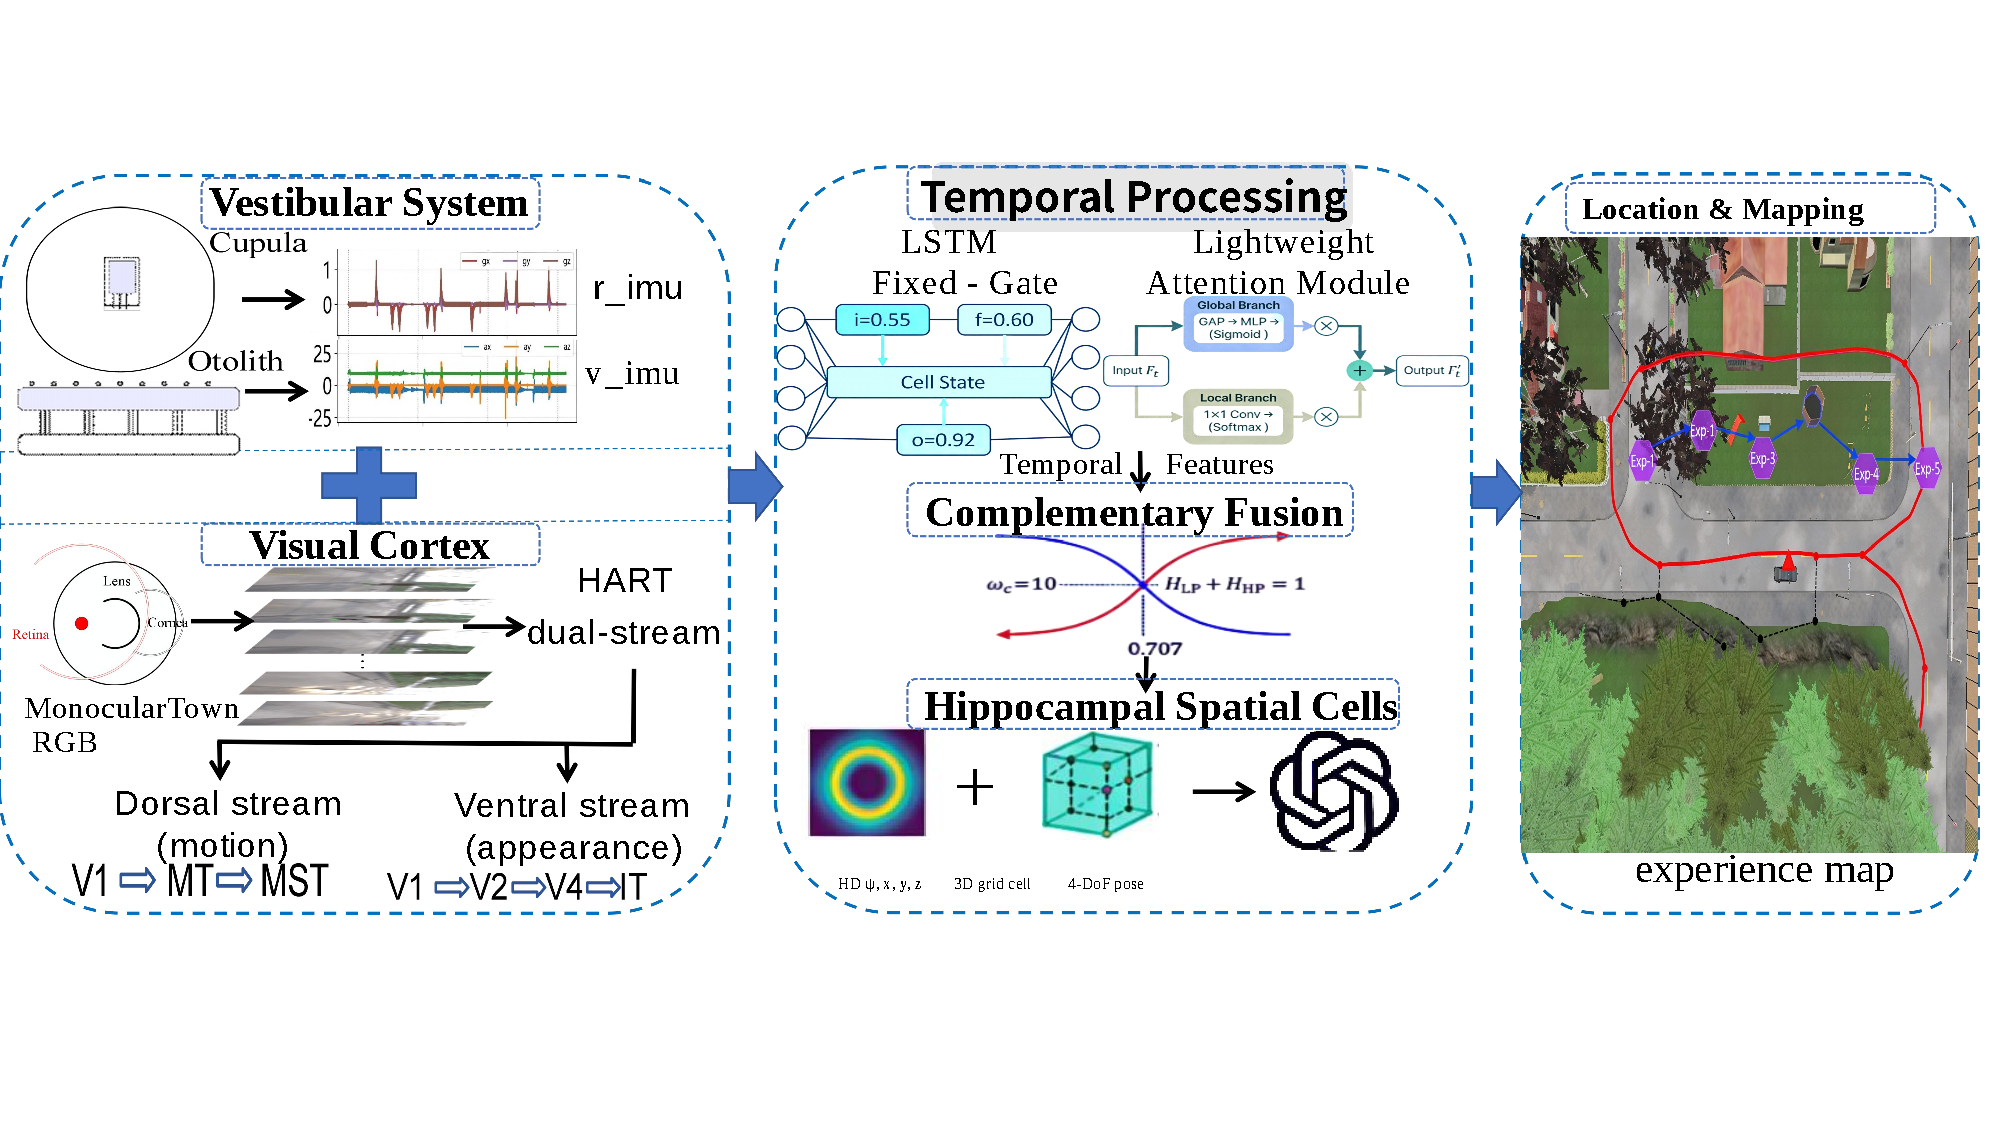
\includegraphics[trim=0pt 97pt 6pt 82pt, clip, width=0.95\textwidth]{fig/2_framework.pdf}
    \caption{Self-contained end-to-end data flow of the proposed multimodal visual-inertial framework. Raw inputs are monocular RGB images and IMU measurements. The visual module splits signals into scene recognition and motion estimation branches; the vestibular module outputs high-frequency inertial motion. Two modalities are fused with the frequency-domain principle of Section~\ref{sec:principle}, instantiated as a fixed-dimension (10-state) EKF. The fused kinematics drive the spatial network to update the unified 4-DoF global state $\mathbf{X}_t$ defined in Eq. \eqref{eq:global_state}. The experience graph module performs loop relaxation to eliminate long-term trajectory drift. All submodules share the standardized state-space variables proposed in this section.}
    \label{fig:system_overview}
\end{figure*}
This work designs a multimodal visual-inertial signal processing system for robot localization, which consists of three tightly coupled functional subsystems: hierarchical multi-scale visual feature operator, vestibular-inertial sensor state estimator, and metric spatial state encoding network. Unlike tightly coupled visual-inertial estimators that augment the state with feature clones, the proposed system keeps a state of fixed dimension and makes the frequency-domain complementarity of the two modalities explicit: the inertial channel supplies the high-frequency prediction, the visual channel supplies gated low-frequency corrections, and the resulting metric state is integrated by a continuous attractor spatial network that suppresses long-term trajectory drift.

\subsubsection{Global Discrete State-Space Model}
To provide a unified mathematical foundation for all subsequent submodule derivations, we first define the discrete state-space representation of the system at time $t$.

1) Multimodal raw input vector
\begin{equation}
    \mathbf{U}_t = \left[ I_t,\, \mathbf{a}_t^\top,\, \boldsymbol{\omega}_t^\top \right]
    \label{eq:input_vec}
\end{equation}
where $I_t$ denotes the captured monocular RGB image; $\mathbf{a}_t$ and $\boldsymbol{\omega}_t$ stand for accelerometer linear acceleration and gyroscope angular velocity measurements, respectively.

2) Core 4-DoF global pose state vector
\begin{equation}
    \mathbf{X}_t = \left[ x_t,\, y_t,\, z_t,\, \psi_t \right]^\top \in \mathbb{R}^3 \times S^1
    \label{eq:global_state}
\end{equation}
In this formulation, $(x_t, y_t, z_t) \in \mathbb{R}^3$ represent global 3D translational coordinates (unit: meter), and $\psi_t \in [-\pi,\pi)$ denotes horizontal yaw angle (unit: radian), i.e.\ the heading is a circular quantity on $S^1$ represented by its $2\pi$-modular angle rather than an element of the rotation group $\mathrm{SO}(2)$.

As visualized in Fig.~\ref{fig:system_overview}, the end-to-end data pipeline consists of five sequential coupled modules:
1. Hierarchical dual-stream visual front-end: Parallel ventral/dorsal branches are constructed to independently generate scene descriptors and compute pixel-wise ego-motion, eliminating mutual interference between recognition and tracking tasks.
2. Vestibular IMU processing module: Derives high-frequency transient motion signals from raw inertial data without iterative online bias calibration.
3. Complementary fusion unit: Adopts first-order IIR filters to separate low-frequency visual drift and high-frequency inertial noise, outputting smoothed translational and rotational kinematics.
4. Metric spatial encoding network: Updates distributed spatial cell states using fused motion cues, and suppresses integral drift via visual template anchoring constraints.
5. Topological experience graph: Records historical visual descriptors and spatial cell snapshots, and executes global graph relaxation once loop closures are detected to guarantee globally consistent metric poses.

\noindent Above this five-module pipeline, the deployed system adds two higher-level corrections that operate on the fused estimate rather than on the raw sensor streams: a monocular scale recovery branch (Section~\ref{sec:scale_recovery}) that drives the EKF's scale state from a lightweight, train-once head over a frozen depth foundation model, and a learned-embedding loop-closure line (Section~\ref{sec:loop_closure}) that re-anchors the trajectory at verified revisits. Both are trained once on simulated data and frozen at deployment, unlike the baseline's kinematic scale observability, which plateaus at the VO-relative scale and recovers no absolute scale. Together they turn the tracking core from an up-to-scale VIO estimator into the metric-scale system evaluated in the experiments.

\subsection{Visual Cortex: Ventral and Dorsal Pathways}
\label{sec:visual_cortex}

The visual front-end (neuroanatomically, the dual ventral, or ``what'', and dorsal, or ``where'', streams of the visual cortex) implements a biologically-plausible processing pipeline inspired by the hierarchical architecture of the primate visual cortex, transforming raw RGB images into compact scene descriptors suitable for place recognition and motion estimation.

\textbf{Hierarchical Feature Extraction.} Given an RGB image $I_t\in\mathbb{R}^{H\times W\times 3}$, we define a sequence of operators that mimic processing stages from retina through inferotemporal cortex.

\textbf{Stages 1--2: Retina, LGN and V1--V4.} Only the last stages of the hierarchy produce quantities the pipeline uses, so the early ones are described rather than modelled. The retinal/LGN stage converts the frame to luminance, applies contrast-limited adaptive histogram equalisation (CLAHE, clip limit $\lambda$) and smooths with a Gaussian kernel $\mathcal{K}_\sigma$; this reproduces centre--surround antagonism without adding tunable parameters. The V1--V4 stage normalises the dynamic range, downsamples to a $12\times16$ map $Z_t$ and removes the map mean, which discards global illumination offsets while preserving layout, the discrete counterpart of divisive normalisation.

\textbf{Stage 3: Inferotemporal (IT) Representation.} The final representation is a compact vectorised descriptor
\begin{equation}
    \boldsymbol{\phi}_t=\mathrm{vec}(Z_t)\in\mathbb{R}^{192},
\end{equation}
whose dimension is fixed by the map size rather than by scene content, analogous to the view-selective, position-invariant representations of IT cortex.

\textbf{Visual Template Matching and Place Recognition.} Place recognition relies on template matching with cosine similarity. This is more robust than intensity metrics such as sum-of-absolute-differences (SAD):
\begin{equation}
    d_{\cos}(\boldsymbol{\phi}_t,\boldsymbol{\phi}_i)=1-\frac{\boldsymbol{\phi}_t^\top\boldsymbol{\phi}_i}{\lVert\boldsymbol{\phi}_t\rVert\,\lVert\boldsymbol{\phi}_i\rVert}
\end{equation}
A new visual template (VT) is created when the current scene is sufficiently different from all existing templates:
\begin{equation}
    \min_{i \in \mathcal{VT}} d_{\cos}(\boldsymbol{\phi}_t, \boldsymbol{\phi}_i)>\tau_{vt},
\end{equation}
with $\tau_{vt}$ set below the OpenRatSLAM default so that similar streets remain distinguishable; the value is an implementation constant reported with the other constants in Section~\ref{sec:experiments}. Template count therefore adapts to how repetitive a route is, which is the mechanism behind the 5-to-964 range measured later.

\textbf{Dual-Stream Architecture and Bio-Inspired Temporal Modeling.} Building upon the hierarchical feature extraction described above, our visual processing incorporates two key bio-inspired innovations: (1) dual-stream architecture mimicking ventral/dorsal path\-ways, and (2) a fixed-coefficient gated filter for temporal coherence without training data requirements.

\textbf{Dual-Stream Visual Processing.}
Following the dual-stream theory of biological vision~\cite{Goodale1992, Mishkin1983}, two channels read the same V1 output and separate layout from appearance. The oriented-gradient channel carries spatial structure and feeds the V1$\rightarrow$V4 stage. The ventral channel carries texture and contrast and stands for V4$\rightarrow$IT:
\begin{align}
    \mathbf{F}^{\text{grad}}_t    & = w_{\parallel} \|\nabla Z_t\| + w_{z} Z_t, \\
    \mathbf{F}^{\text{ventral}}_t & = w_{v} Z_t + w_{t} \sigma_{\text{local}}(Z_t) + w_{c} \mathcal{C}_\lambda(Z_t),
\end{align}
where $\sigma_{\text{local}}$ is the local standard deviation and $\mathcal{C}_\lambda$ the CLAHE operator already used at the retinal stage. In the first channel the gradient magnitude plays the role of orientation-selective simple-cell responses and the weighted sum aggregates them into a compact layout map; the second channel weights appearance, texture and contrast in that order, mimicking V4 selectivity and IT invariance. The weights $(w_{\parallel},w_z)$ and $(w_v,w_t,w_c)$ are fixed implementation constants shared by every scene, settings rather than fitted parameters, and no scene-specific tuning is applied.

The dual streams are then integrated through a lightweight global-local feature modulation mechanism that approximates self-attention effects using global statistics rather than full Query-Key-Value operations, maintaining $\mathcal{O}(N)$ complexity for real-time per\-for\-mance.

\textbf{Fixed-Coefficient Gated Filter for Zero-Shot Temporal Modeling.}
Unlike conventional data-driven LSTMs that must be trained on domain-specific data, our temporal module is a gated recurrence whose three gates (input $i_0$, forget $f_0$ and output $o_0$) are constants held for every sequence, chosen once from the vestibular--visual integration literature~\cite{Angelaki2004, Cullen2012}: $i_0$ and $f_0$ weigh new evidence against retained context, and $o_0$ close to unity keeps the response dominated by the current frame. No gate transformation and no input matrix is learned.

This design offers three critical advantages for SLAM applications:

\textbf{(1) Zero-shot deployment capability:} No training data is required, so the filter can be deployed in a new environment immediately. That matters because every environment has its own visual statistics and collecting representative training data is impractical. All five evaluation sequences, four simulated and one real, run with the same constants and no environment-specific tuning.

\textbf{(2) Biological interpretability:} The three constants map onto empirically documented principles. A forget gate around one half implements short-term spatial memory retention consistent with hippocampal replay dynamics, where recent experience is preferentially kept for path integration; an output gate near unity prioritises current sensory input, mimicking the vestibular emphasis on immediate self-motion cues; and the balanced input gate trades novelty detection against stability.

\textbf{(3) Computational efficiency:} No backpropagation and no gradient computation, while the reference implementation holds 39--76~FPS on CPU; constant gates also map directly onto hardware (FPGAs, neuromorphic chips) with no weight storage or update logic.

The filter processes fused gradient-ventral features sequentially, maintaining a cell state $\mathbf{C}_t$ and a hidden state $\mathbf{h}_t$. Because the gates are constants and the input connection is the identity, this recurrence reduces to a first-order infinite-impulse-response (IIR) filter, the degenerate member of the LSTM family. The gate vocabulary above is kept only to make that correspondence explicit.

\textbf{Comparison with Learning-Based Approaches.} Section~\ref{sec:experiments} compares the fixed-coefficient filter against NeuroSLAM's learned LSTM under one evaluation protocol. The point is not that constants beat learning in general, but that when the task structure matches the biological mechanism, a principled constant-coefficient design can hold its own while remaining deployable without training.

\textbf{Visual Motion Extraction.} In addition to scene recognition, the visual front-end extracts ego-motion cues from inter-frame correspondences, mimicking dorsal-stream processing in area MST.

\textbf{Sparse Correspondences and Relative Pose.} Each frame contributes $N$ ORB keypoints with rotated-BRIEF descriptors. Matches pass a mutual nearest-neighbour test with the Lowe ratio and are lifted to bearing vectors with the inverse intrinsic matrix. The essential matrix follows from a RANSAC-wrapped minimal solver on the epipolar constraint and is decomposed into the inter-frame rotation and a unit translation direction. The yaw increment comes from the ZYX decomposition of that rotation with a gimbal-lock guard. Robustness is enforced twice, at the descriptor level for uniqueness and then at the geometric level for consensus, and the consensus set doubles as the degeneracy test used below.

\textbf{Scale Ambiguity and Observation Injection.} The decomposed translation is unit-norm: it fixes direction and never magnitude. The metric displacement over one interval is therefore $\Delta\mathbf{p}^{\mathrm{vis}}_t = s_t\,\hat{\mathbf{t}}_t$, where $s_t=\exp(x_{10,t})$ is the tenth state of Eq.~\eqref{eq:state} (Section~\ref{sec:scale_recovery}); one symbol $s$ denotes this quantity throughout. Below a minimum inlier count the frame is not admitted as a motion measurement, and the zero-displacement placeholder enters the filter with inflated noise, acting as a no-motion prior. Otherwise the inlier count $n_{\mathrm{inl}}$ yields a quality factor $q_f=\clip(n_0/n_{\mathrm{inl}},\,1/3,\,3)$ that multiplies the observation covariance together with a smooth residual factor, clamped to $[0.008,10]$ (Section~\ref{sec:deployed_filter}).

Beyond this motion stream, the front-end also supplies the pixel-level metric depth field $\hat z_t$ and the learned scene embeddings $\boldsymbol{e}_t$ used by the two higher-level corrections. The motion pathway never consumes depth, and both are inferred asynchronously and cached outside the real-time path.

\subsection{Vestibular System}
\label{sec:vestibular}

The vestibular front-end processes inertial measurements to extract self-motion cues analogous to the mammalian ves\-tib\-u\-lar system. The ves\-tib\-u\-lar apparatus comprises semicircular canals (angular velocity) and otolith organs (linear acceleration).

\textbf{Angular Velocity Extraction.} From the gyroscope measurements $\mathbf{g}_t\in\mathbb{R}^3$ (IMU frame), we use the raw $z$-axis gyro. A constant bias is estimated once from the static start-up window and subtracted thereafter (Section~\ref{sec:fusion}); no per-frame bias estimation is performed. For 4-DoF lo\-cal\-i\-za\-tion-and-map\-ping under a planar constraint, the yaw (azimuthal) angular velocity is approximated by
\begin{equation}
    r_t \approx \mathbf{e}_z^\top\,\boldsymbol{\omega}_t^g,\quad \mathbf{e}_z=(0,0,1)^\top.
\end{equation}
where $\boldsymbol{\omega}_t^g$ is raw gyroscope angular velocity vector measured by IMU, and $\mathbf{e}_z$ is unit vertical basis vector.
This corresponds to the horizontal semicircular canal cue, adequate for our complementary fusion with vision.

\textbf{Linear Acceleration Usage.} For a planar 4-DoF state only two inertial quantities matter beyond yaw: an along-track speed and a vertical speed. The reference implementation derives indicative versions of both by removing the gravity magnitude $g$ from the measured specific force and integrating over the frame interval $\Delta t$ with constant gains $\kappa_t$ and $\kappa_z$,
\begin{equation}
    \hat v_{t} = \kappa_t\big(\lVert\mathbf{a}_t\rVert - g\big)\Delta t,
    \qquad
    \hat v_{z,t} = \kappa_z\big(a_{t,z} - g\big)\Delta t,
\end{equation}
where $\mathbf{a}_t$ is the accelerometer reading and $g$ the gravitational acceleration. The construction is crude by design: it carries no bias state and no gravity-vector estimate, because its only role is to give the reference implementation a high-frequency channel. The deployed filter takes the same band from the IMU propagation of Section~\ref{sec:deployed_filter}. The consequences of treating $g$ as a constant are examined as a failure mode in Section~\ref{sec:failure_analysis}.

\textbf{Bias Estimation.} The accelerometer and gyroscope biases that enter the kinematic cues are estimated once, in the static start-up window of each sequence (the first 200 samples with the platform at rest), and are then held constant; no online gravity-vector estimation is performed and a constant gravity magnitude is used for specific-force compensation. This keeps the front-end free of extra filter states and is sufficient at the 20\,Hz CARLA cadence (KITTI~07 is processed at its native $\approx$9.6\,Hz, $\Delta t\approx0.104$\,s); the residual effect of a fixed gravity magnitude is analyzed as a failure mode in the discussion.

\subsection{Vestibular--Visual Fusion: Frequency-Domain Principle and Deployed Filter}
\label{sec:fusion}

\textbf{How NeuroLocMap operates.} The modules of the framework are coupled in one direction only, so the operating chain can be stated before the equations. For every camera frame $t$: (1) the visual front-end returns a relative displacement, a yaw increment and an inlier count; (2) the filter is propagated IMU-step by IMU-step across the inter-frame interval with \eqref{eq:ekf_pred}--\eqref{eq:ekf_cov}; (3) the gated corrections of Table~\ref{tab:gates} are applied in a fixed order of velocity amplitude, attitude, scale and position, because each branch supplies a quantity that a later one consumes (the position anchor is expressed in metres through the scale state, and the velocity amplitude is compared in the same units); the heading branch of the table is implemented but disabled in the configuration that produced all reported numbers, so the chain above runs on four active branches; (4) the filtered pose is published and, in EKF-odometry mode, handed to the spatial layer as its motion source; (5) the grid-cell attractor integrates the frame-to-frame displacement into a bump of activity and the head-direction layer carries the yaw (Section~\ref{sec:grid_cells}); (6) when the current visual template and spatial code are novel, an experience node is created and linked to its predecessor (Section~\ref{sec:loop_closure}); (7) an accepted loop-closure event relaxes a drift field over the stored trajectory and re-anchors the path integrator. Steps (1)--(4) constitute the filter, and steps (5)--(7) act on its output without writing back into it.

The frequency split assigns each modality the band in which it is reliable: visual odometry for slow, accurate motion and inertial integration for fast transients. Neither channel is treated as an absolute observation of comparable confidence, so the filter avoids arbitration between them and requires no joint optimization over visual features. The state is held at 10 dimensions, so the per-update cost does not grow with the number of tracked features, and any branch can be disabled without perturbing the others (Section~\ref{sec:deployed_filter}). No downstream stage feeds back into the filter, so the ablation in Section~\ref{sec:ablation} isolates each module rather than describing correlations. All results reported in this paper are produced by the deployed 10-state filter. The fixed-weight combination of the reference implementation is retained only as an ablation reference and as the subject of per-module timing measurements. Sections~\ref{sec:scale_recovery}--\ref{sec:loop_closure} follow the same order for each step: input, computation, output.

\begin{figure*}[!t]
    \centering
    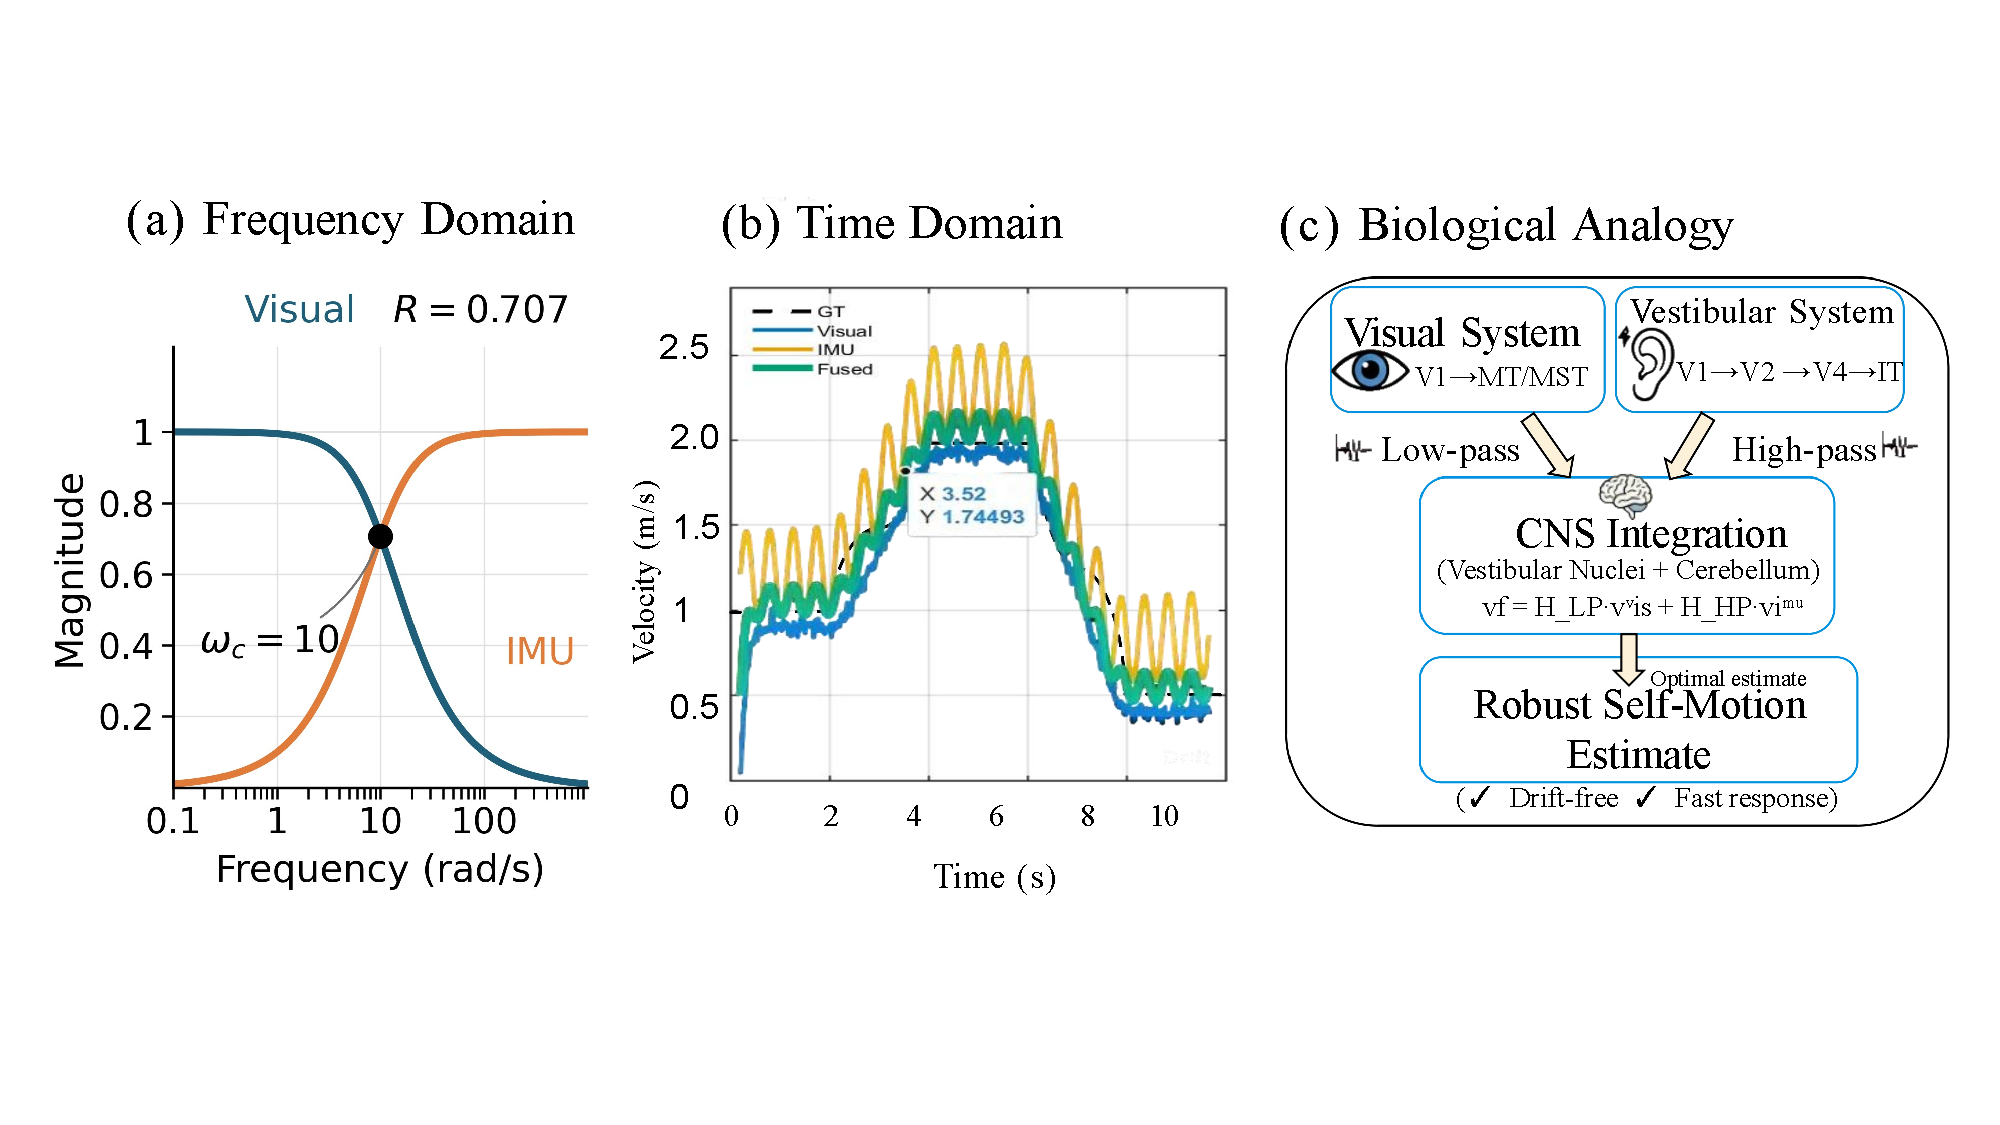
\includegraphics[trim=12pt 107pt 20pt 98pt, clip, width=\textwidth]{fig/imu_visual_complementary_fusion.pdf}
    \caption{Frequency-domain principle of the vestibular--visual fusion. (a) Frequency-domain analysis of the complementary low- and high-pass characteristics. (b) Time-domain signal comparison. (c) Biological analogy to ves\-tib\-u\-lar--visual integration in the CNS. (a)--(c) illustrate the principle of Section~\ref{sec:principle}; the deployed filter that produces all reported results is specified in Section~\ref{sec:deployed_filter}.}
    \label{fig:imu_visual_fusion}
\end{figure*}

\subsubsection{Biological Principle and Frequency-Domain Complementarity}
\label{sec:principle}

\textbf{Filter Design.} Let $\mathcal{L}_\tau$ denote a low-pass filter with time constant $\tau$, and $\mathcal{H}_\tau$ the complementary high-pass filter satisfying $\mathcal{L}_\tau+\mathcal{H}_\tau=\mathrm{Id}$, with $\mathrm{Id}$ the identity operator. Realized recursively,
\begin{equation}
    L_t = \alpha_{\mathrm{iir}} L_{t-1} + (1-\alpha_{\mathrm{iir}}) x_t,\qquad L_0=0 \label{eq:lowpass}
\end{equation}
where $\alpha_{\mathrm{iir}}$ is the IIR forgetting factor and $L_t$ the low-frequency smoothed signal.

\textbf{Biological Analogy.} This is the discrete counterpart of multisensory integration in the ves\-tib\-u\-lar nuclei and posterior parietal cortex (area~7a), where visual and ves\-tib\-u\-lar signals are combined to estimate self-motion; neurons in these regions exhibit weighted combinations of the two tuning profiles, with dynamic weighting according to signal reliability.

\textbf{Discrete-Time Implementation.} With sampling interval $\Delta t$ we implement first-order IIR filters and set the forgetting factors from the target time constants, $\alpha_{\mathrm{iir}}=\exp(-\Delta t/\tau)$ and $\alpha_{r,\mathrm{iir}}=\exp(-\Delta t/\tau_r)$, so that the analogue cut-off is reproduced at the 20\,Hz cadence used here.

\textbf{Frequency-Domain Transfer Functions.} In the Laplace domain with $s_{\mathrm{lap}}=j\omega$ the two filters satisfy $H_{LP}(s_{\mathrm{lap}})+H_{HP}(s_{\mathrm{lap}})=1$ (unity gain at all frequencies). The cut-off $\omega_c=1/\tau$ separates the two regions: for $\omega\ll\omega_c$, $|H_{LP}|\approx1$ and $|H_{HP}|\approx0$, so the visual pathway dominates (drift-free, slower dynamics); for $\omega\gg\omega_c$ the IMU cues dominate (fast but drifting). With $\tau=0.1$\,s the cut-off is $\omega_c=10$\,rad/s ($\approx1.6$\,Hz), so that IMU handles high-frequency motion ($>2$\,Hz: vibration, rapid turns) while vision corrects low-frequency drift ($<1$\,Hz). This mimics ves\-tib\-u\-lar--visual integration, where ves\-tib\-u\-lar organs respond in 0.1--10\,Hz and visual motion perception dominates below 0.5\,Hz~\cite{Angelaki2004}.

\subsubsection{Temporal Alignment}
\label{sec:alignment}

In the CARLA synchronous acquisition setting (20\,Hz, $\Delta t=0.05$\,s) both sensors are driven by a single cadence, and a lightweight aligner pairs each camera frame with the nearest IMU sample within a 0.02\,s tolerance using greedy one-to-one matching (each IMU sample is consumed at most once). Timestamps of the aligned streams were checked frame by frame over all 5000 CARLA frames and the 1101 KITTI~07 frames, with no gaps and no dropped frames, so the fusion operates on pre-aligned samples and requires no intra-frame interpolation.

\subsubsection{Deployed Implementation: Total-State EKF with Error-State Covariance}
\label{sec:deployed_filter}

\textbf{State.} The deployed fusion core is a total-state EKF whose covariance is propagated in error-state form, with state
\begin{equation}
    \mathbf{x}_t=\big[x,y,z,\ v_x,v_y,v_z,\ \phi,\theta,\psi,\ \log s_t\big]^{\!\top}
    \label{eq:state}
\end{equation}
i.e.\ position, velocity, Euler attitude and a tenth state $\log s_t$, the online scale that links the VO frame to the metric world (notation of Section~\ref{sec:notation}; the scale branch is detailed in Section~\ref{sec:scale_recovery}). The tenth state is what makes the other nine interpretable in metres: without it the visual channel would only be consistent up to scale.

\textbf{Prediction.} Between observations the state is propagated by IMU kinematics,
\begin{equation}
\begin{aligned}
    \mathbf{a}^{w}_t &= R(\boldsymbol{\Theta}_t)\big(\mathbf{a}_t-\mathbf{b}_a\big)+\mathbf{g}_w,\qquad \mathbf{g}_w=[0,0,-g]^{\top},\\
    \boldsymbol{\Theta}_{t+1} &= \wrap\big(\boldsymbol{\Theta}_t+(\boldsymbol{\omega}_t-\mathbf{b}_g)\Delta t\big),\\
    \big(v^{x}_{t+1},v^{y}_{t+1}\big) &= \big(v^{x}_t,v^{y}_t\big)+\big(a^{w,x}_t,a^{w,y}_t\big)\Delta t,\qquad v^{z}_{t+1}=0,\\
    \big(p^{x}_{t+1},p^{y}_{t+1}\big) &= \big(p^{x}_t,p^{y}_t\big)+\big(v^{x}_t,v^{y}_t\big)\Delta t,\qquad z_{t+1}=z_t,
\end{aligned}
    \label{eq:ekf_pred}
\end{equation}
with $R(\cdot)$ the body-to-world rotation, $\wrap(\cdot)$ mapping an angle to $(-\pi,\pi]$, $g$ constant, and $\mathbf{b}_a,\mathbf{b}_g$ fixed from the static start (Section~\ref{sec:vestibular}). Three properties of this form are deliberate rather than incidental. (i) The vertical channel is \emph{frozen}: the vertical velocity is clamped to zero after every prediction and the altitude is held at its initial value, so the filter propagates exactly the planar 4-DoF motion model assumed in Section~\ref{sec:framework_arch}, and this clamp is what keeps the planar VO increments and the tenth scale state mutually consistent. (ii) Integration is explicit in the current velocity; no $\tfrac12\mathbf{a}\Delta t^{2}$ term is used, so the position Jacobian contains only $\partial p^{x}/\partial v^{x}=\partial p^{y}/\partial v^{y}=\Delta t$ and the attitude block of $\mathbf{F}$ is the identity, which keeps the Jacobian sparse and cheap to form. (iii) The attitude is propagated with the gyroscope only; the visual attitude branch of Table~\ref{tab:gates} corrects it downstream. The covariance follows
\begin{equation}
    \mathbf{P}_{t+1}=\mathbf{F}_t\mathbf{P}_t\mathbf{F}_t^{\top}+\mathbf{Q}_c\,\Delta t,
    \label{eq:ekf_cov}
\end{equation}
with process noise and initial covariance fixed once for all sequences,
\begin{equation}
\begin{aligned}
    \mathbf{Q}_c&=\mathrm{diag}\big(0.18,0.18,0.09,\ 0.72,0.72,0.36,\\
    &\qquad\qquad 7.2\mathrm{e}{-3},7.2\mathrm{e}{-3},1.8\mathrm{e}{-2},\ 2.0\mathrm{e}{-5}\big),\\
    \mathbf{P}_0&=\mathrm{diag}\big(2,2,0.5,\ 2,2,1,\ 0.05,0.05,0.05,\ 0.64\big),
\end{aligned}
\end{equation}
ordered as $(p,v,\Theta,\log s)$: the entries of $\mathbf{Q}_c$ carry the units $\mathrm{m^2\,s^{-1}}$, $\mathrm{m^2\,s^{-3}}$, $\mathrm{rad^2\,s^{-1}}$ and $\mathrm{s^{-1}}$ (the tenth state is $\log s$, dimensionless, so its noise density is per second), and those of $\mathbf{P}_0$ the units $\mathrm{m^2}$, $\mathrm{m^2\,s^{-2}}$, $\mathrm{rad^2}$ and $1$; the scale variance $0.64$ corresponds to the $\sigma_0=0.8$ log prior, and $\log s$ starts at $0$ (unit scale). A pure-IMU dead-reckoning copy is maintained in parallel for diagnostic purposes; it is not used as a comparison row in the experiments.

\textbf{Gated Observation Update.} Each branch produces an innovation $\mathbf{y}=\mathbf{z}-h(\hat{\mathbf{x}})$ with $\mathbf{S}=\mathbf{H}\mathbf{P}\mathbf{H}^{\top}+\mathbf{R}_{\mathrm{obs}}$, accepted only if
\begin{equation}
    \mathbf{y}^{\top}\mathbf{S}^{-1}\mathbf{y}<\chi^2(d;\alpha_\chi).
    \label{eq:gate}
\end{equation}

The branches, their models and the deployed thresholds are listed in Table~\ref{tab:gates}, and they are applied in the order of the table for the dependency reason given above. Branch~1 (disabled in the deployed runs, Table~\ref{tab:gates}) would recover yaw from turn kinematics: on frames with mean speed $>3$\,m/s, $|a_\perp|>0.3$\,m/s$^2$ and $|\omega_z|<1.2$\,rad/s, the ratio $a_\perp/|v|$ is integrated onto a heading base that is independent of both the gyroscope and the current heading estimate, giving a yaw-angle observation with a per-frame step limit of 0.26\,rad ($\approx15^{\circ}$). Branch~4 is a dual-path, log-domain scale observation: the calibrated depth scale of Section~\ref{sec:scale_recovery} takes precedence and is frozen inside a 0.30 dead band in the log domain ($\approx1.35\times$; used for all reported runs and set as the released-code default); the kinematic cue $|a_\perp|/(|\omega|v)$ is used whenever the depth path is unavailable, skipped or gated out. Each active branch carries its own observation model, gate threshold and residual window, and no branch observes a quantity from the same signal that it later corrects, which is why the four active gates are tested separately within one frame rather than jointly.

\begin{table}[!htbp]
    \centering
    \caption{Observation branches of the 10-state fusion core. Branches~2--5 are applied in this order and are those used in all reported runs; branch~1 is implemented but disabled in that configuration (see the table note).}
    \label{tab:gates}
    \footnotesize
    \begin{tabularx}{\textwidth}{@{}c >{\RaggedRight\arraybackslash}X c c c c@{}}
        \toprule
        \# & Observation $\mathbf{z}$ (dim) & $h(\hat{\mathbf{x}})$ & $\chi^2(d;\alpha_\chi)$ & $\mathbf{R}_{\mathrm{obs}}$ \\
        \midrule
        1$^{\dagger}$ & yaw from $\int a_\perp/|v|\,\mathrm{d}t$ (turn frames), (1) & $\psi$ & 3.84 (1;0.95) & $0.05$ \\
        2 & VO displacement over $\Delta t_{\mathrm{eff}}$, scaled by $s$, on heading, (1) & $\lVert\mathbf{v}\rVert$ & 9.21 (2;0.99) & $0.20$ \\
        3 & roll/pitch from vestibular cue, (2) & $(\phi,\theta)$ & 9.21 (2;0.99) & diag$(0.05,0.50)$ \\
        4 & log-scale: depth median or $|a_\perp|/(|\omega|v)$, (1) & $\log s$ & 6.63 (1;0.99) & $0.05$ (depth) / $0.02$ (kin.) \\
        5 & re-anchored VO increment $\times s$, 30 frames, (2) & $(x,y)$ & 13.82 (2;0.999) & diag$(0.06,0.06)$ \\
        \bottomrule
    \end{tabularx}

    \vspace{2pt}
    {\footnotesize $\Delta t_{\mathrm{eff}}$ denotes the measured inter-frame interval actually spanned by the VO increment (not a nominal frame period). Branch~1$^{\dagger}$ is implemented and documented for completeness, but its flag is off in the configuration that produced \emph{every} reported number, so the deployed filter runs branches~2--5 only; it is included in the table because the released code contains it, not because it contributes to the results. Branch~5 is accompanied by a weak height prior ($R=25$\,m$^2$). Branch~2 applies the 2-dof threshold to a scalar residual (deliberately permissive). Each $\mathbf{R}_{\mathrm{obs}}$ is scaled by the quality factor of Section~\ref{sec:deployed_filter}; thresholds and covariances were fixed before the ablation runs and are identical across the five sequences.}
\end{table}

\textbf{Quality-Adaptive Noise.} The VO inlier count $n_{\mathrm{inl}}$ gives $q_f=\operatorname{clip}(60/n_{\mathrm{inl}},\tfrac13,3)$, and the smooth residual factor comes from the mean of that branch's last 10 Mahalanobis distances, $\rho=\operatorname{clip}\big(q_f[\,0.05+(d/5d_{\mathrm{of}})^{1.5}\,],0.008,10\big)$; the nominal covariance of Table~\ref{tab:gates} is multiplied by $\rho$. Degraded frames thus contribute less and degenerate frames contribute nothing beyond an inflated no-motion prior.

\textbf{Numerical Stability and Ablation Integrity.} All updates use the Joseph form with post-update regularisation (symmetrisation plus a minimum-eigenvalue clamp), so the covariance stays positive definite over the 5000-frame CARLA collection runs (KITTI~07 is 1101 frames) without reinitialisation. Because each branch is an independent gated term with its own observation model, gate threshold and residual window, disabling one leaves the other branches' formulations untouched; the single coupling runs through the tenth state, which the scale-branch ablation isolates by construction. This is what makes the ablation matrix of Section~\ref{sec:ablation} interpretable rather than merely descriptive.

\subsubsection{Computational Cost}
\label{sec:cost}

The deployed filter carries a fixed $10\times10$ covariance, so each update is a constant-size operation, $\mathcal{O}(10^{3})$, independent of the number of visual features. Filters that augment the state with feature clones (MSCKF, VINS-Mono) pay $\mathcal{O}(Nn^{3})$. Per-module timings on the MATLAB front-end are reported in Table~\ref{tab:runtime}.

\subsubsection{Reference Implementation: Fixed-Weight Combination (Ablation Only)}
\label{sec:reference_impl}

The MATLAB reference implementation realizes the principle of Section~\ref{sec:principle} directly as a fixed-weight convex combination with binary activity gating, using $\eta=0.3$ for translation, $\eta_r=0.7$ for yaw and $0.5$ for height, with the fallback cue taken from the gravity-compensated specific-force magnitude when the visual channel is inactive. The weights and clamps were fixed once and kept identical across all sequences, with no per-sequence tuning. This component serves as the fixed-weight reference in the ablation and as the object of the runtime measurements, and is not the source of the main results. Its per-update cost is $\mathcal{O}(1)$ with two scalar states per fused channel, which makes it the lightest element of the pipeline.

\subsection{Monocular Scale Recovery Branch}
\label{sec:scale_recovery}

\textbf{Problem.} The tenth state $\log s$ is driven by two cues: turn kinematics, observable only in turning frames (294/1101 frames on KITTI~07) and, by construction, recovering only the \emph{VO-relative} scale, and, in the deployed configuration, the calibrated depth path of this section, which takes precedence whenever it is available (Section~\ref{sec:deployed_filter}). Neither cue determines the absolute scale between the visual frame and the metric world on its own. Monocular metric-depth networks offer an independent cue, but their zero-shot predictions carry a scene-dependent bias (a preliminary study showed the raw depth scale to be unreliable across scenes), so raw depth cannot serve directly as a scale observation. Rather than trusting the depth network, we learn a lightweight \emph{calibration} that maps depth-statistics features to the true global scale: trained once on simulation, frozen at deployment.

\textbf{Operation.} The branch runs per inter-frame interval, not per IMU step. For each interval the frozen depth model emits one metric depth map; eight depth statistics are formed from it and median-smoothed over $W{=}50$ intervals; the head returns a single log-scale prediction, and a sliding median of those predictions is compared with the filter state. Only outside the 0.30 dead band of Section~\ref{sec:deployed_filter} does the result enter branch~4 of Table~\ref{tab:gates}. The head is therefore never a pose estimator: it contributes one scalar at a small fraction of the frame rate, cannot move the trajectory by itself, and is bypassed whenever it is unavailable or its innovation is gated out.

\textbf{Structure.} For each frame $t$, let $\hat z_t$ denote the metric depth map predicted by a frozen monocular depth foundation model (Depth-Anything-V2, outdoor head). We summarize it into an 8-dimensional feature vector
\begin{align}
    \mathbf{f}_t = \big[&\log \hat s^{\,\mathrm{dav2}}_t,\ \log d^{\mathrm{med}}_t,\ \log (d^{\mathrm{std}}_t{+}\epsilon),\ \log d^{\mathrm{p10}}_t,\ \log d^{\mathrm{p90}}_t, \nonumber\\
    &\log (\hat s^{\,\mathrm{inl}}_t{+}1),\ f_x/W,\ 1\big]^{\top},
    \label{eq:scale_feat}
\end{align}
where $\hat s^{\,\mathrm{dav2}}_t$ is the windowed-median zero-shot depth scale estimate (VO displacement over median metric depth over the inter-frame interval); $d^{\mathrm{med}}, d^{\mathrm{p10}}, d^{\mathrm{p90}}, d^{\mathrm{std}}$ are the metric-depth median, percentiles, and standard deviation; $\hat s^{\,\mathrm{inl}}_t$ is the feature-inlier-consistent scale; and $f_x/W$ encodes the camera geometry. A windowed median ($W{=}50$ intervals) smooths each feature. The scale head $g_\theta$ is a compact MLP $8{\to}64{\to}64{\to}1$ (ReLU, ${\sim}4.8$k parameters) that predicts the log scale
\begin{equation}
    \hat \ell_t = g_\theta(\mathbf{f}_t) \;\approx\; \log s^{*}_t,
    \label{eq:scale_head}
\end{equation}
supervised, during training only, by the per-interval ground-truth scale
\begin{equation}
    \ell^{*}_t = \log \frac{\lVert \mathbf{p}^{*}_t - \mathbf{p}^{*}_{t-1} \rVert}{\lVert \mathbf{p}_t - \mathbf{p}_{t-1} \rVert},
    \label{eq:scale_sup}
\end{equation}
where $\mathbf{p}^{*}$ are ground-truth metric positions (available in simulation) and $\mathbf{p}$ the VO positions.

\textbf{Train-Once Protocol.} The head is optimized on three simulated towns (Town05/03/07) with Adam (learning rate $10^{-3}$, weight decay $10^{-3}$), MSE loss on standardized features, and early stopping on a held-out split ($10\%$); the feature standardization is frozen together with the weights. A fourth town (Town10HD) is held out entirely, and no real-world data is seen. After training, \emph{all parameters are frozen}. There is no per-sequence calibration and no online adaptation at deployment, and the head is used as-is on every test sequence.

\textbf{Gated Integration.} The prediction $\hat s_t = \exp(g_\theta(\mathbf{f}_t))$ enters the EKF as the scale-branch observation in the log domain: it (i) replaces the depth-median initialization of $\log s$ when the branch activates, (ii) persistently pulls the scale state through a chi-square-gated update with a log-domain dead band, and (iii) suppresses the kinematic scale observation while active, so the two scale evidences do not fight. The correction is \emph{scale-only} by design. It adjusts the 10th state and, through it, the visual-velocity observations, and it never rewrites position or attitude directly. A wrong scale prediction therefore degrades gracefully instead of corrupting the fused trajectory.

\textbf{Zero-Shot Behavior and Honest Limits.} Within the simulation domain the learned mapping generalizes across scenes, including the held-out town, and outperforms an ordinary-least-squares calibration baseline on all five evaluation sequences. Across the sim-to-real boundary, however, the mapping does not transfer. On KITTI~07 the head predicts a scale correction in the wrong direction ($s\approx0.3$ where the route requires $\approx1.8$), and deploying it degrades the EKF (Supplementary Section~S.1 quantifies this failure). All real-world results in this paper therefore run without the scale branch, a limitation we return to in the experiments. The head's computational cost is negligible: ${\sim}4.8$k parameters and sub-millisecond CPU inference per frame, outside the real-time critical path. The frozen depth backbone is evaluated asynchronously and cached.

\subsection{Entorhinal Cortex: Grid Cells and Head Direction Cells}
\label{sec:grid_cells}

The spatial representation module (neuroanatomically, the entorhinal cortex, whose grid cells and head-direction cells provide the brain's metric coordinate system) encodes the robot's 4-DoF pose through bio-inspired neural coordinate systems using conjunctive pose cells. The 3D location $(x, y, z)$ is represented by grid cells using a 3D multi-dimensional continuous attractor network (MD-CAN), while orientation $\psi$ (yaw) is encoded by multilayered head direction cells. These representations enable stable, noise-tolerant path integration through attractor dynamics.

\textbf{3D Grid Cell Network.} The 3D grid cell network draws on the 3D spatial representations found in the mammalian brain, in particular the 3D grid cells discovered in the bat entorhinal cortex~\cite{finkelstein2016three} and the periodic grid structure characterized in rodents~\cite{hafting2005microstructure}, to encode position and provide a metric substrate for path integration. Our implementation realizes this representation as a 3D continuous attractor network that extends 2D attractor dynamics to full 3D space through separable Gaussian excitation--inhibition connectivity on a cubic cell lattice with toroidal wrapping, preserving metric path integration and noise resilience.

\textbf{Network Architecture.} The 3D grid cell network is a 3D multi-dimensional continuous attractor network (MD-CAN) with dimensions $N_x \times N_y \times N_z$ ($N_x = N_y = N_z = 36$ in our implementation). The network activity $\mathbf{A}^\mathrm{g}_t \in \mathbb{R}^{N_x \times N_y \times N_z}$ represents a distributed population code for the robot's 3D position $(x_t, y_t, z_t)$, where each cell $(i,j,k)$ is tuned to a preferred spatial location within the environment. The activity forms a localized ``bump'' (or activity packet) centered at the current position, analogous to the activity bump observed in rodent entorhinal cortex recordings.

The network's topology implements periodic boundary conditions with toroidal wrapping, enabling unbounded spatial representation. Connectivity is local and separable along the three axes: each cell excites a Gaussian neighborhood of $7\times7\times7$ cells ($\sigma = 1.5$ cells per axis) and inhibits a $5\times5\times5$ neighborhood with a broader spread ($\sigma = 2$ cells per axis), and both kernels wrap toroidally so that activity packets move seamlessly across boundaries. This local excitation--inhibition structure sustains a single stable bump and supports continuous 3D path integration.

\begin{figure*}[!t]
    \centering
    \includegraphics[width=\textwidth]{fig/3d_grid_cell_network.pdf}
    \caption{3D grid cell network. (a) 3D activity packet representing position $(x,y,z)$ through distributed population code. (b) Separable Gaussian excitation kernel ($7\times7\times7$ cells, $\sigma=1.5$ cells per axis) with toroidal wrapping. (c) 4-DoF encoding scheme combining position and heading representations.}
    \label{fig:3D_grid_cell_network}
\end{figure*}

Figure~\ref{fig:3D_grid_cell_network} schematically illustrates: (a) the 3D activity bump at position $(x, y, z)$, represented as isosurfaces to visualize the localized excitation; (b) the separable Gaussian excitation kernel and its toroidal wrapping on the cubic cell lattice; (c) the complete 4-DoF encoding pipeline integrating position and heading representations.

\textbf{Continuous Attractor Dynamics.} The network maintains a localized ``bump'' of activity through three key mechanisms:

\textbf{(1) Local excitation.} Cells excite their neighbors according to a Gaussian connectivity kernel. With a separable kernel
\begin{equation}
    \mathcal{K}^\mathrm{g}_{a,b,c}=\mathcal{N}(a;0,\sigma_x)\mathcal{N}(b;0,\sigma_y)\mathcal{N}(c;0,\sigma_z)
\end{equation}
where $\mathcal{N}(\cdot;\mu,\sigma)$ denotes one-dimensional Gaussian distribution, and $\sigma_x,\sigma_y,\sigma_z$ are spatial kernel widths along three axes.
the excitatory update is:
\begin{equation}
    \Delta A^\mathrm{g}_{i,j,k}=\sum_{p,q,r} A^\mathrm{g}_{p,q,r}\,\mathcal{K}^\mathrm{g}_{\langle i-p\rangle_{N_x},\langle j-q\rangle_{N_y},\langle k-r\rangle_{N_z}}
\end{equation}
where $\langle \cdot \rangle_N$ denotes modulo-$N$ wrapping for periodic boundary conditions. In our implementation $\sigma_x = \sigma_y = \sigma_z = 1.5$ cells with a $7\times7\times7$ kernel.

\textbf{(2) Global inhibition and normalization.} Uniform global inhibition subtracts a fixed threshold $\theta_g$ with rectification, which suppresses weak background activity while preserving the bump:
\begin{equation}
    A^\mathrm{g}_{i,j,k}\leftarrow \big[A^\mathrm{g}_{i,j,k}+\Delta A^\mathrm{g}_{i,j,k}-\theta_g\big]_+,\quad [\cdot]_+ = \max(0, \cdot)
\end{equation}
In our implementation $\theta_g = 2\times10^{-4}$. After inhibition, the activity is $L_1$-normalized:
\begin{equation}
    A^\mathrm{g}\leftarrow \frac{A^\mathrm{g}}{\lVert A^\mathrm{g}\rVert_1}=\frac{A^\mathrm{g}}{\sum_{i,j,k}|A^\mathrm{g}_{i,j,k}|}
\end{equation}
This normalization ensures the activity pattern has unit total mass, making the readout (center of mass) insensitive to overall activity magnitude.

\textbf{(3) Path integration.} The activity bump shifts according to fused velocity cues $\mathbf{v}^\mathrm{f}_t = (v^f_x, v^f_y, v^f_z)$. Index shifts are computed as:
\begin{equation}
    (\Delta i,\Delta j,\Delta k)=\big(\lfloor \gamma_x v^f_x\Delta t\rfloor,\ \lfloor \gamma_y v^f_y\Delta t\rfloor,\ \lfloor \gamma_z v^f_z\Delta t\rfloor\big)
\end{equation}
where $\gamma_x,\gamma_y,\gamma_z$ are metric-to-index gain factors converting physical velocity to network grid shifts.
\begin{equation}
    A^\mathrm{g}_{i,j,k}\leftarrow A^\mathrm{g}_{\langle i-\Delta i\rangle_{N_x},\langle j-\Delta j\rangle_{N_y},\langle k-\Delta k\rangle_{N_z}}
\end{equation}
This discrete shifting operation efficiently implements path integration on the toroidal network topology.

\textbf{Visual Anchoring and Drift Correction.} Pure path integration accumulates drift over time. To prevent unbounded error, the grid cell activity is anchored to visual landmarks through a static, creation-time association: each visual template $m$ records the grid-cell coordinates $(g^x_m,g^y_m,g^z_m)$ and head-direction heading of its creation instant, i.e., the path-integration state at that moment. When template $m$ is matched by a later frame, corrective activity is injected at its recorded coordinates:
\begin{equation}
    \Delta A^\mathrm{g}_{g^x_m,g^y_m,g^z_m} \mathrel{+}= E_0\cdot\frac{30-e^{1.2 d_m}}{30},\qquad d_m\in[0,d_{\max}]
\end{equation}
where $E_0$ is the baseline injection energy and $d_m$ is the template activity level: it is reset to the cap $d_{\max}$ upon each match and decays linearly over time. The injected amplitude grows as a template remains unmatched for longer, from $\approx E_0/3$ at $d_m=d_{\max}$ toward $E_0$ as $d_m\to 0$. This decayed, weak injection is a RatSLAM-style anti-capture design: a single spurious match (e.g., during agent stasis) cannot capture the grid-cell network; a consistent injection from multiple visual templates is required to form an effective anchoring.

In the final system configuration this template-level injection pathway is deactivated (the deployed visual-template implementation never clears its first-match flag, so the injection condition is never met); visually driven drift correction in the deployed system is carried entirely by the anchoring--re-anchoring mechanism of the experience map.

\textbf{Multilayered Head Direction Cells.} The multilayered head direction cell (HDC) network represents the robot's orientation using a 2D MD-CAN with dimensions $N_\psi \times N_h$ (azimuth bins by height layers). Different height layers allow representation of heading at various vertical positions, supporting 3D operation where orientation may vary with altitude.

\textbf{Network Architecture.} The multilayer head-direction network has activity $\mathbf{A}^\mathrm{h} \in \mathbb{R}^{N_\psi \times N_h}$ ($N_\psi = 36$ azimuth bins and $N_h = 36$ height layers in the released configuration, i.e.\ a $10^{\circ}$ azimuth bin). Each cell $(u, h)$ is tuned to azimuth angle $\theta_u = 2\pi u / N_\psi$ and height layer $h$.

\textbf{Attractor Dynamics.} Similar to the grid cell network, the HDC network employs local excitation, global inhibition, and path integration. With a Gaussian kernel $\mathcal{K}^\mathrm{h}$:
\begin{equation}
    \Delta A^\mathrm{h}_{\psi,h}=\sum_{u,v}A^\mathrm{h}_{u,v}\,\mathcal{K}^\mathrm{h}_{\langle \psi-u\rangle_{N_\psi},\langle h-v\rangle_{N_h}}
\end{equation}
followed by fixed-threshold global inhibition ($\theta_h = 2\times10^{-4}$, the same rectify-and-subtract form as above) and $L_1$ normalization:
\begin{equation}
    A^\mathrm{h}\leftarrow \frac{\tilde{A}^\mathrm{h}}{\lVert \tilde{A}^\mathrm{h}\rVert_1},\qquad \tilde{A}^\mathrm{h}=\big[A^\mathrm{h}+\Delta A^\mathrm{h}-\theta_h\big]_+
\end{equation}
Path integration shifts the activity bump according to yaw rate $r^f$ and vertical velocity $v^f_z$:
\begin{equation}
    \Delta\psi=\lfloor \gamma_\psi r^f \Delta t\rfloor,\quad \Delta h=\lfloor \gamma_h v^f_z \Delta t\rfloor
\end{equation}
where $\gamma_\psi$ converts angular velocity to azimuth bins, and $\gamma_h$ maps vertical velocity to height layer shifts. The gains follow directly from the cell sizes of the released implementation (Table~\ref{tab:gains}): with the toroidal network wrapping every $2\pi$ in the angular axes, one azimuth bin corresponds to $10^{\circ}$ and the height-layer and grid-$z$ spacings are $2\pi/36\approx0.17$~m; the planar grid axes are metric at $1$~m per cell (a 36-cell toroidal period).

\begin{table}[!htbp]
    \centering
    \caption{Path-integration gains and cell sizes of the spatial layers (values from the released implementation; the height channels are nominal because the deployed filter freezes the vertical channel).}
    \label{tab:gains}
    \footnotesize
    \begin{tabular}{@{}llll@{}}
        \toprule
        Axis & Gain & Cell size & Toroidal period \\
        \midrule
        Grid $x,y$ & $\gamma_x=\gamma_y=1$ cell/m & 1 m & 36 m \\
        Grid $z$ & $\gamma_z=36/(2\pi)\approx5.73$ cells/m & $\approx0.17$ m & $\approx6.3$ m \\
        HD azimuth & $\gamma_\psi=36/(2\pi)\approx5.73$ bins/rad & $10^{\circ}$ & $360^{\circ}$ \\
        HD height & $\gamma_h=36/(2\pi)\approx5.73$ layers/m & $\approx0.17$ m & $\approx6.3$ m \\
        \bottomrule
    \end{tabular}
\end{table}
\textbf{Pose Readout.} The metric pose estimate is decoded from the spatial cell activities via center-of-mass computation (population vector decoding):
\begin{align}
    \hat{\mathbf{p}}_t & = ({\hat x}_t, {\hat y}_t, {\hat z}_t) = \frac{\sum_{i,j,k} \mathbf{c}_{i,j,k} A^\mathrm{g}_{i,j,k,t}}{\sum_{i,j,k} A^\mathrm{g}_{i,j,k,t}}, \quad \mathbf{c}_{i,j,k} = (x_i, y_j, z_k) \\
    \hat{\psi}_t       & = \mathrm{\mathrm{atan2}}\left(\sum_{u,h} A^\mathrm{h}_{u,h,t} \sin\theta_u, \sum_{u,h} A^\mathrm{h}_{u,h,t} \cos\theta_u\right), \quad \theta_u = 2\pi u / N_\psi
\end{align}
This decoding naturally handles the circular topology of orientation (using $\mathrm{\mathrm{atan2}}$ to avoid angle wrapping issues) and provides sub-bin resolution for position through the weighted average.

\textbf{Where the Spatial Layer Sits.} The grid-cell and head-direction layers are not a second estimator. They consume the filtered pose (frame-to-frame displacement and yaw in EKF-odometry mode), integrate it into a bump of activity, and expose the resulting spatial code for experience creation, with the head-direction layer supplying the yaw channel of the 4-DoF code. Decoding the bump returns a pose that gates novelty and defines loop constraints but does not correct the filter. The attractor dynamics therefore stabilise the representation rather than revise the estimate. This directionality, from filter to spatial code to constraints to output trajectory, keeps the layer biologically interpretable without turning it into a competing estimator.

\subsection{Hippocampal Experience Map and Loop Closure}
\label{sec:loop_closure}

In the brain, the hippocampus links place representations into episodic memories of traversed space, and their replay and re-consolidation underpin memory-guided navigation. The multilayered experience map mirrors this organization: it represents 3D spatial experiences as a graph structure, providing a hybrid topological-metric representation that combines the benefits of discrete place-based maps (topological robustness, loop closure) and continuous metric representations (accurate localization).

\textbf{Experience Representation.} Each experience node $\mathcal{E}_i$ encodes a distinct spatial episode comprising the active visual template and descriptor $(VT_i,\,\boldsymbol{\phi}_i\in\mathbb{R}^{192})$, the concurrent spatial-cell codes $\mathbf{P}^{gc}_i=\mathbf{A}^\mathrm{g}_i\in\mathbb{R}^{N_x\times N_y\times N_z}$ and $\mathbf{P}^{hdc}_i=\mathbf{A}^\mathrm{h}_i\in\mathbb{R}^{N_\psi\times N_h}$, the metric pose $(x_i, y_i, z_i, \psi_i)$ decoded from these activities, and the timestamp $t_i$ for temporal ordering.
This rich multimodal encoding enables robust loop closure detection through visual matching while maintaining metric information through the spatial cell codes.

\textbf{Experience Creation and Linking.} As the robot navigates, new experiences are created when the current spatial representation differs sufficiently from all existing experiences. The creation criterion combines visual and spatial cell similarity:
\begin{equation}
    \begin{aligned}
        \text{Create new experience if }\; & d_{cos}(\boldsymbol{\phi}_t, \boldsymbol{\phi}_j) > \tau_{VT} \quad \text{for all } j \in \mathcal{E} \\
                                           & \text{or } \lVert (\hat{x}_t, \hat{y}_t, \hat{z}_t) - (x_j, y_j, z_j) \rVert > d_{thresh}
    \end{aligned}
\end{equation}
where $\tau_{VT} = 0.08$ is the visual template matching threshold and $d_{thresh}$ is a spatial distance threshold (typically 0.5~m).

Consecutive experiences are linked by directed edges encoding the relative pose transition:
\begin{equation}
    \boldsymbol{\delta}_{i \to i+1} = (\Delta x, \Delta y, \Delta z, \Delta \psi) = (x_{i+1} - x_i, y_{i+1} - y_i, z_{i+1} - z_i, \psi_{i+1} - \psi_i)
    \label{eq:edge}
\end{equation}
These edges form the primary topological structure of the experience map graph $\mathcal{G} = (\mathcal{V}, \mathcal{E})$.

\textbf{Loop Closure Detection.} Loop closure is detected when the current visual template matches a previous experience beyond a minimum temporal separation (to avoid trivial closures):
\begin{equation}
    \begin{aligned}
        \text{Loop closure detected if } \exists j:\; & d_{cos}(\boldsymbol{\phi}_t, \boldsymbol{\phi}_j) < \tau_{loop} \\
                                                      & |t - t_j| > T_{min}
    \end{aligned}
\end{equation}
where $\tau_{loop} = 0.05$ (stricter than the template creation threshold to reduce false positives) and $T_{min} = 50$ frames (2.5\,s at the 20\,Hz CARLA cadence of Section~\ref{sec:alignment}; 5.2\,s at the 9.6\,Hz KITTI~07 rate).

Upon detecting a loop closure, a loop edge is added to the graph with the pose residual:
\begin{equation}
    \mathbf{T}_{loop} = (\hat{x}_t - x_j, \hat{y}_t - y_j, \hat{z}_t - z_j, \hat{\psi}_t - \psi_j)
    \label{eq:loopres}
\end{equation}
This loop constraint typically violates graph consistency (due to accumulated drift), triggering map relaxation.

\textbf{Map Relaxation.} Map relaxation distributes the loop closure error across all experiences along the loop path to minimize global inconsistency. We employ an iterative relaxation algorithm:

\textbf{Step 1: Identify loop path.} Given a loop closure edge from experience $j$ to experience $t$, identify the sequence of experiences $\mathcal{P} = \{j, j+1, \ldots, t-1, t\}$ along the path.

\textbf{Step 2: Compute pose residual.} The increments accumulated along the loop should reproduce the loop-closure residual; any mismatch is the drift to be removed:
\begin{equation}
    \mathbf{e}_{loop} = \sum_{k \in \mathcal{P}} \boldsymbol{\delta}_{k \to k+1} - \mathbf{T}_{loop}
\end{equation}
where $\boldsymbol{\delta}_{k \to k+1}$ is the 4-DoF increment of Eq.~\eqref{eq:edge}, $\mathbf{T}_{loop}$ is the loop-closure residual of Eq.~\eqref{eq:loopres}, and $\mathcal{P}$ is the ordered sequence of experiences along the loop. Both terms live in the same $(x,y,z,\psi)$ parameterization, so the subtraction is well defined. The residual is nonzero whenever the increments accumulated along the loop disagree with the visual match, which is the case that triggers relaxation.
\textbf{Step 3: Distribute correction.} Distribute the correction proportionally across the loop experiences:
\begin{equation}
    \boldsymbol{\delta}_{k \to k+1} \leftarrow \boldsymbol{\delta}_{k \to k+1} - \frac{1}{|\mathcal{P}|}\mathbf{e}_{loop}
\end{equation}
Even distribution assumes that drift accumulates at a constant rate. Because the increments are treated as vectors, this composition is first-order in yaw; corrections that exceed this regime are applied by the Sim(3) re-anchoring operator described below.

\textbf{Step 4: Update experience poses.} Recompute all experience poses by integrating the corrected transitions:
\begin{equation}
    \mathbf{X}_{k+1} = \mathbf{X}_{k} + \boldsymbol{\delta}_{k \to k+1}
\end{equation}
consistent with the increment definition of Eq.~\eqref{eq:edge}.

\textbf{Step 5: Re-anchor spatial cells.} Inject the corrected pose $(\hat{x}, \hat{y}, \hat{z}, \hat{\psi})_{corr}$ back into the spatial cell networks by reinitializing the activity bumps at the corrected locations. This ``resets'' the path integration from the corrected reference, preventing error accumulation in subsequent operation.

This relaxation procedure runs iteratively until convergence or a maximum number of iterations, ensuring the experience map remains globally consistent while preserving local metric accuracy.

\textbf{Deployed Loop-Closure Line: Frame-Based Candidates.} The formulation above describes the node-level reference map. Every loop result reported in this paper comes from the frame-level line specified here, which detects loops over \emph{frames} rather than experience nodes. Each frame is described by a frozen DINOv2-S global scene embedding $\mathbf{e}_t$, refined by a fine-tuned head trained under the same train-once protocol as the scale branch, on simulation data only. A candidate match for the current frame is the historical frame $j^{*} = \arg\max_{j} \cos(\mathbf{e}_t, \mathbf{e}_j)$, restricted to frames whose EKF-odometry arc-length separation exceeds $\mathrm{arc}_{\min}$ (50~m). That arc-length criterion replaces the $T_{\min}$ frame gap of the node-level formulation. It removes trivial self-matches while keeping the search exhaustive over the plausible far-history. This frame-level candidate stage decouples loop detection from experience-node creation and gives the gate chain dense per-frame evidence.

\textbf{Four-Gate Chain.} A candidate becomes an accepted loop event only if it passes four fixed gates (all thresholds set once across all five scenarios):
\begin{align}
    \mathrm{accept}(t, j^{*}) \iff{}
    & \cos(\mathbf{e}_t, \mathbf{e}_{j^{*}}) \ge \tau
    \;\wedge\; \mathrm{streak}(t, j^{*}) \ge 15 \nonumber\\
    &\;\wedge\; |\Delta\psi_{t j^{*}}| \le 60^{\circ}
    \;\wedge\; \lVert \mathbf{c}_{t j^{*}} \rVert \le 25\,\mathrm{m},
    \label{eq:pr_gates}
\end{align}
with a cumulative correction budget $\sum_i \lVert \mathbf{c}_i \rVert \le 35$~m across the trajectory and deduplication of historical anchors (each past frame anchors at most once). The \emph{similarity gate} ($\tau = 0.94$) is calibrated by a five-scenario sweep: observed false candidates score 0.907--0.935 while strong genuine revisits score $\ge 0.949$. The \emph{persistence gate} ($\ge 15$ consecutive candidate frames, $\pm 10$ tolerance) exploits a structural property of genuine revisits. A vehicle traversing the same street produces a sustained streak of high-similarity frames, whereas perceptual aliasing produces single-frame or short-burst excursions. This gate is scale-free and transfers across domains unchanged. The \emph{orientation gate} ($60^{\circ}$ heading difference) admits same-direction and moderately oblique re-visits while rejecting reversed trajectories and geometrically implausible matches. The correction budget bounds the damage of any single wrong acceptance. The chain is conservative on purpose. On KITTI~09 its sole genuine loop lies in the final two frames, where the streak can reach only $2 < 15$ and the gate correctly declines; releasing it in hindsight would change the error by merely $-0.12$~m. The orientation gate rejects that sequence's two high-similarity but geometrically inconsistent candidates (Supplementary Section~S.3). Silence is preferred to a wrong re-anchor.

\textbf{Injection.} An accepted event injects a one-shot translation correction $\mathbf{c}_{t j^{*}}$ (step size $\beta = 1.0$) that pulls the current segment toward the matched node's map pose, writes a link edge into the experience graph, and hands the event to the full-Sim(3) re-anchoring operator described below. The corrected segment then enters the drift-field relaxation above.

\textbf{Distributed Closure Drift Field.} Each re-anchoring event (a loop closure or a match to an existing node) resets the incremental dead-reckoning state, so the raw output trajectory contains a discrete correction step of $\mathbf{c}_i$ at frame $f_i$. These steps form an accumulated staircase $\mathbf{C}_{\mathrm{cum}}(f)$ whose discrete jumps are the dominant source of per-frame inconsistency between the experience-map-corrected output and the filtering front-end. We therefore relax each step into a continuous drift field, inspired by slow re-consolidation of spatial memory in the hippocampal--entorhinal system. For every recorded re-anchoring pulse $\mathbf{c}_i$ at frame $f_i$ with $\lVert\mathbf{c}_i\rVert \le C_{\max}$, a raised-cosine ramp of duration $W_i$ is applied:
\begin{equation}
    F_i(f) =
    \begin{cases}
        \tfrac{1}{2}\bigl(1-\cos(\pi (f-f_i)/W_i)\bigr), & f_i \le f < f_i + W_i \\
        1, & f \ge f_i + W_i
    \end{cases}
\end{equation}
and the corrected trajectory is
\begin{equation}
    \hat{\mathbf{p}}(f) = \mathbf{p}_{\mathrm{exp}}(f) + \Bigl(\sum_i F_i(f)\,\mathbf{c}_i \;-\; \sum_{i:\,f_i \le f}\mathbf{c}_i\Bigr),
\end{equation}
so each correction persists (the held level $\mathbf{c}_i$ is retained after the ramp) but its onset is smoothed over $W_i$ frames, and the staircase $\mathbf{C}_{\mathrm{cum}}$ is exactly replaced by the continuous field. Three design choices, validated by offline parameter sweeps on all five outdoor sequences, shape the field:
\begin{itemize}
    \item \textbf{Adaptive relaxation time.} $W_i = \mathrm{clip}(W_0 + W_{\perp}\,\lVert\mathbf{c}_i\rVert,\; W_0,\; W_{\max})$: larger jumps relax more slowly, analogous to the slower re-consolidation of stronger spatial memories and to the longer time constants of grid-cell drift correction. Released values (closed-loop benchmark configuration): $W_0 = 100$ frames, $W_{\perp} = 0$ frames/m, $W_{\max} = 4000$ frames, $C_{\max} = 2.0$~m; the per-sequence sweep of Section~\ref{sec:experiments} varies $W_0 \in [100, 2400]$ frames, $W_{\perp} \in [0, 80]$ frames/m and $C_{\max} \in [2, 6]$~m.
    \item \textbf{Tail completion.} Each ramp is truncated at the trajectory end ($W_i \leftarrow \min(W_i, f_{\mathrm{end}}-f_i+1)$) so that the drift field is fully relaxed by the final frame, avoiding a half-relaxed ramp that would leave terminal bias.
    \item \textbf{Amplitude gating.} Jumps with $\lVert\mathbf{c}_i\rVert > C_{\max}$ are applied instantaneously and excluded from the field: large corrections correspond to distant true loop closures whose early node positions are trustworthy, whereas small corrections (nearby re-visits, hash collisions) are uncertain and benefit from slow relaxation. Sweeps show that flattening \emph{all} steps degrades accuracy (e.g., Town01: +0.64\% RMSE), while gating yields per-frame RMSE improvements over both the un-relaxed baseline and the EKF front-end on all five sequences.
\end{itemize}
With the EKF-odometry mode ($\mathrm{NLM\_USE\_EKF\_ODO}$) the experience map consumes the fused EKF trajectory as its motion source (frame-to-frame displacement and yaw increments), and new experience nodes are pinned to the EKF map coordinates, so the grid-cell path integrator and the experience graph operate on a common, tightly constrained metric ground truth; the drift field then corrects only the residual re-anchoring steps on top of this unified foundation.

\textbf{Closed-Loop Full-Sim(3) Re-Anchoring.} Each re-anchoring pulse above translates the subsequent trajectory but does not change its global scale or orientation, so the monocular scale ambiguity keeps accumulating between loops. We therefore complement it with a loop-triggered operator: at every accepted loop-closure event at frame $t_{\mathrm{now}}$, a full similarity transform is fitted between the \emph{anchor window} $\mathbf{A}$ (the first $\mathrm{win}$ moving frames of the trajectory, after the static prelude) and the \emph{current window} $\mathbf{C}$ (the $\mathrm{win}$ frames ending at $t_{\mathrm{now}}$, capped by the next event) by a Procrustes fit
\begin{equation}
    \mathbf{A} \approx \sigma_{\mathrm{sim}}\,(\mathbf{C}\mathbf{R}_{P}) + \mathbf{t}, \qquad \sigma_{\mathrm{sim}} \in [0.05,\,20],
\end{equation}
with $\mathrm{win} = 250$ frames (self-calibrated by an offline window sweep) and the scale gate rejecting degenerate fits. The entire segment after $t_{\mathrm{now}}$ (up to the next event) is then pulled back into the anchor frame,
\begin{equation}
    \hat{\mathbf{p}}(f) = \sigma_{\mathrm{sim}}\,(\mathbf{p}(f)\mathbf{R}_{P}) + \mathbf{t}, \qquad t_{\mathrm{now}} < f < t_{\mathrm{next}},
\end{equation}
applied independently per event on the pre-correction trajectory (non-chained, so one event's refit is not polluted by its predecessor's transform). Because each accepted loop is a genuine re-visit of the same physical location, the re-anchoring is a global consistency correction that uses no ground-truth information; on loop-free routes it is a strict no-op.



%% ==================== EXPERIMENT ====================
% float placement parameters are defined once in NeuroSLAM_KBS.tex (compact layout)
% rewritten 2026-10-16: the paper's main configuration is the NLM full system (EKF tracking core + scale branch + loop line);
% five sequences = CARLA Town05/03/07/10HD + KITTI07; both calibers (sim3_full upper bound / rigid SE(3));
% numbers come from final_metrics.json / se3_metrics.json (τ=0.94 solution, full-system trajectories).

\section{Experiments and Results}
\label{sec:experiments}

We evaluate NeuroLocMap on five scenarios spanning simulated urban driving (CARLA Town05/03/07/10HD) and real-world highway driving (KITTI~07). The full system couples the vestibular-visual EKF core with two higher-level corrections: an online monocular scale branch (a lightweight regression head over a frozen depth foundation model, trained once on simulated data and frozen at deployment), and an experience-map loop-closure line built on learned scene embeddings. All higher-level components are \emph{trained once on simulation} and deployed \emph{zero-shot} on every test sequence, including the real-world one.

\subsection{Experimental Setup and Datasets}

\textbf{Implementation Details.} All experiments are conducted on a single laptop workstation (Intel Core i9-14900HX CPU, 32~GB RAM, NVIDIA GeForce RTX 5070 Laptop GPU); the entire SLAM pipeline runs on CPU, and no GPU is used anywhere in the reported results. The LSTM temporal module uses manually-tuned fixed gate values (input=0.5, forget=0.5, output=0.9) rather than learned parameters. Measured end-to-end throughput of the reference implementation (including final evaluation and plotting) is 67--76~FPS on the four CARLA towns and 39~FPS on KITTI~07, whose denser map (964 templates) makes template matching the dominant growing cost.

\textbf{Baseline Methods.} We compare NeuroLocMap against four baselines. EKF core only is the same 10-state filter of Section~\ref{sec:deployed_filter} with the deep scale head and the experience map disabled. It is an ablation of our spatial modules, not a separate method. VO is ORB-based monocular visual odometry with epipolar pose recovery (Essential matrix $+$ \texttt{recoverPose}), without inertial fusion or loop closure. EKF+scale drives the same filter's scale state from the head of Section~\ref{sec:scale_recovery} with no loop closure, which isolates the scale branch. The loop-closure line alone completes the set. Per-branch parameters of the shared filter are those of Table~\ref{tab:gates} and are not re-tuned per baseline.

\textbf{Implementation-Level Fairness.} For all methods, we use the same synchronized sensor streams and timestamps. Baseline trajectories are generated by our Python pipeline: on CARLA they are recorded during data collection (the EKF fusion baseline to fusion\_pose.txt, the VO baseline to visual\_odometry.txt, and the ground truth to ground\_truth.txt); on KITTI~07 the same EKF/VO pipeline is run offline on the raw public sequence with identical configuration. The evaluation then loads these trajectories and compares them against NeuroLocMap under identical sequences, ensuring differences reflect al\-go\-rith\-mic design rather than data or timing mismatches. All reported CARLA numbers correspond to data collected with the final EKF implementation (single global hyper-parameter set shared by all maps; collection parameters as specified in Table~\ref{tab:datasets}), so the numbers in Table~\ref{tab:results} are reproducible from the asset bundle described in the Data availability statement for the shipped artifacts, and the carried cells are marked in the repository's REPRODUCE.md.

\textbf{Evaluation Datasets.} We evaluate on five diverse scenarios across two benchmark datasets (Table~\ref{tab:datasets}): (1) CARLA Simulation, four towns (Town05, Town03, Town07 and Town10HD): simulated urban driving scenarios~\cite{dosovitskiy2017carla} with ground-truth poses and synchronized IMU-camera data, all re-collected with the same protocol and background traffic. Town05 (486~m) is the loop-richest route, crossing the same commercial streets repeatedly; Town03 (474~m) threads narrow alleys with strong viewpoint changes; Town07 (618~m) is a low-texture suburban loop; Town10HD (452~m) is an open layout with essentially a single revisit. (2) KITTI Odometry Sequence 07~\cite{geiger2012kitti}: real-world highway driving (692~m, 1101 frames) with high-quality visual features and limited loop opportunities, challenging systems on medium-length real-world trajectories.

\begin{table*}[!t]
    \centering
    \setlength{\tabcolsep}{2.8pt} % slightly tighter column separation
    \footnotesize
    \caption{Dataset Characteristics and Evaluation Scenarios. All CARLA scenarios were re-collected with the final EKF implementation at a commanded speed of 12~km/h and with background traffic (20 autopilot vehicles + 20 kinematically driven pedestrians); frames are logged at 20~Hz and include the stationary start-up window and slow turning segments, so the mean along-route speed is below the commanded value (6.5--8.9~km/h realized across the four towns); KITTI is a fixed public benchmark. ``Accepted links'' counts the loop-closure edges admitted by the persistence and orientation gates.}
    \label{tab:datasets}
    \begin{tabular}{@{}llccl@{}}
        \toprule
        Dataset  & Environment & Length & Frames & Characteristics                    \\
        \midrule
        Town05   & Urban mixed & 486~m  & 5000   & Loop-rich route, 7 accepted links  \\
        Town03   & Urban alleys& 474~m  & 5000   & Narrow streets, viewpoint changes, 7 links \\
        Town07   & Suburban loop& 618~m & 5000   & Low-texture residential loop, 7 links \\
        Town10HD & Urban open  & 452~m  & 5000   & Open layout, single revisit, 1 link \\
        KITTI~07 & Highway     & 692~m  & 1101   & Real-world open trajectory, 11 map links \\
        \bottomrule
    \end{tabular}
\end{table*}

\textbf{Evaluation Metrics and Alignment Calibers.} We use the standard SLAM metrics: Absolute Trajectory Error (ATE, RMSE after alignment)~\cite{sturm2012benchmark}, terminal drift rate (terminal error normalized by trajectory length), and Relative Pose Error (RPE, frame-to-frame consistency). NeuroLocMap recovers the metric scale online, so the alignment protocol is itself part of the claim. We therefore evaluate every method under two calibers, each estimated over the full trajectory and applied consistently to all methods. The first is a full Sim(3) refit (rotation, translation and one global scale, Umeyama/Procrustes). Its fitted scale absorbs any global scale error by construction, so it measures trajectory shape and serves as an upper bound for every method. The second is an SE(3) rigid alignment (Kabsch, rotation and translation only, no scale). A trajectory with a wrong metric scale cannot be rescued by this aligner, so the caliber directly tests metric-scale recovery. Our metric-localization claim is stated in the SE(3) caliber, where NeuroLocMap beats the EKF without any post-hoc fitting. We do not claim a globally scale-perfect system. Residual global scale errors remain, with Sim(3)-fitted factors between 0.79 and 1.92 across scenarios, so the Sim(3) numbers should be read as the shape-only upper bound.

\subsection{Performance Results and Analysis}

\textbf{Quantitative Performance.} Table~\ref{tab:results} presents the quantitative comparison under both calibers. NeuroLocMap (full system) \emph{outperforms the 10-state EKF visual-inertial baseline on all five scenarios under both calibers}: by $+$16.5\% (KITTI~07) to $+$59.3\% (Town05) under the Sim(3) upper bound, and by $+$1.5\% (KITTI~07, the thinnest margin) to $+$33.9\% (Town05) under the SE(3) rigid caliber --- where an unrecovered metric scale cannot be absorbed by the aligner. The \emph{scale branch is the dominant contributor}: driving the EKF's scale state with the deep scale head alone (EKF+scale, no loop closure) already removes 13.1--32.7\% of the EKF's SE(3) error and 22.4--54.8\% of its Sim(3) error, and the full system adds a further loop-closure margin on Town05 ($-2.03$~m Sim(3)) and Town03 ($-0.76$~m). Against monocular VO, the full system wins on all five scenarios by $+$33.7\% to $+$68.8\% (Sim(3)). Two honest caveats accompany these headline numbers. First, on Town07 the scale branch \emph{alone} is the strongest configuration (27.90/29.21~m vs 28.75/31.51~m for the full system): the loop's marginal contribution there is slightly negative ($+0.85$~m), which we analyze in Section~\ref{sec:failure_analysis}. Second, on KITTI~07 the scale head does not transfer zero-shot to real imagery (Supplementary Section~S.1), so no EKF+scale row exists there and the KITTI result is carried by the loop-closure line alone; the ``full system'' row on KITTI~07 therefore denotes the loop line over the EKF core, with the scale branch deliberately inactive (Supplementary Section~S.1), and we label it as such rather than reporting a re-tuned variant.

\begin{table*}[!t]
    \centering
    \setlength{\tabcolsep}{3pt}
    \footnotesize
    \caption{Quantitative Performance Comparison Under Two Alignment Calibers (ATE RMSE, m)}
    \label{tab:results}
    \begin{threeparttable}
        \footnotesize
        \setlength{\tabcolsep}{3.5pt}
        \begin{tabular}{@{}l cccc cccc@{}}
            \toprule
            & \multicolumn{4}{c}{Sim(3) full refit (shape-only upper bound)} & \multicolumn{4}{c}{SE(3) rigid (metric-scale caliber)} \\
            \cmidrule(lr){2-5} \cmidrule(lr){6-9}
            Dataset & Ours & EKF+scale & EKF & VO & Ours & EKF+scale & EKF & VO \\
            \midrule
            Town05   & \textbf{18.07} & 20.10 & 44.44 & 48.26 & \textbf{32.67} & 33.26 & 49.40 & 53.86 \\
            Town03   & \textbf{15.31} & 16.07 & 23.36 & 49.10 & \textbf{17.31} & 17.47 & 23.53 & 49.15 \\
            Town07   & 28.75 & \textbf{27.90} & 40.64 & 50.07 & 31.51 & \textbf{29.21} & 42.85 & 50.13 \\
            Town10HD & \textbf{14.44} & \textbf{14.44} & 18.61 & 35.86 & \textbf{49.88} & 49.89 & 57.38 & 58.04 \\
            KITTI~07 & \textbf{18.45} & n/a              & 22.09 & 27.84 & \textbf{29.99} & n/a              & 30.45 & 38.35 \\
            \bottomrule
        \end{tabular}
        \begin{tablenotes}
            \scriptsize
            \item Bold = best of the four configurations in that caliber. NeuroLocMap outperforms the EKF on all five scenarios under both calibers (Sim(3) $+$16.5\% to $+$59.3\%; SE(3) $+$1.5\% to $+$33.9\%) and monocular VO on all five (Sim(3) $+$33.7\% to $+$68.8\%).
            \item \emph{Anchored Sim(3) caliber} (closed-loop benchmark only): both trajectories are anchored at the loop event, and the reported quantity is the terminal displacement between them.
            \item Drift rates (terminal error / length): NeuroLocMap 2.9--11.7\% (Sim(3)) and 0.2--15.2\% (SE(3)), versus 1.6--13.3\% and 5.0--19.0\% for the EKF and 9.9--24.2\% and 13.7--17.2\% for VO.
            \item n/a: the zero-shot scale head is not deployed on KITTI~07 (real-image domain gap; Supplementary Section~S.1); the KITTI result is the loop-closure line over the EKF core. On Town07 the scale branch alone is strongest (loop contribution $+0.85$~m); elsewhere the full system is best.
        \end{tablenotes}
    \end{threeparttable}
\end{table*}

\textbf{Performance by Scenario Type.} On the four CARLA towns (452--618~m), NeuroLocMap cuts the EKF's error by 22.4\% (Town10HD) to 59.3\% (Town05) under Sim(3), and by 13.1\% to 33.9\% under SE(3), while cutting monocular VO's error by 42.6--68.8\%.

On the real-world 692~m highway (KITTI~07), NeuroLocMap runs with the loop-closure line over the EKF core (the zero-shot scale branch is disabled; Supplementary Section~S.1) and still outperforms the EKF by 16.5\% under Sim(3) (18.45~m vs 22.09~m) and by 1.5\% under SE(3) (29.99~m vs 30.45~m), while beating monocular VO by 33.7\% (27.84~m). This validates that the vestibular-visual core plus learned loop closure remains effective on real-world driving --- and quantifies how much of the framework's simulated-data advantage currently survives the domain gap.

\textbf{Representative Performance Analysis.} Figure~\ref{fig:representative_performance} visualizes two representative scenarios: Town05 (486~m, loop-rich mixed urban) and Town10HD (452~m, open layout). The top row shows per-method metrics (RMSE, drift, RPE, and template/loop counts); the bottom row shows the aligned per-frame position error evolution. On Town05, NeuroLocMap reaches 18.07~m RMSE --- 59.3\% better than the EKF (44.44~m) and 62.6\% better than monocular VO (48.26~m, whose drift reaches 24.2\% versus 4.6\%) --- while its experience map holds 175 nodes over 175 visual templates with 7 accepted links. On Town10HD, it reaches 14.44~m versus 18.61~m for the EKF ($+$22.4\%) and 35.86~m for VO ($+$59.7\%); the map holds 481 nodes but only a single accepted link, and the EKF+scale row (14.44~m) shows that essentially the entire gain comes from the scale branch, the loop being inert on this open layout. These two cases bracket the framework's operating regime: loop-rich urban driving, where experience-based re-anchoring adds global consistency on top of the metric-scale correction, and open layouts, where the system reduces to EKF+scale. Comprehensive results for all five datasets are given in Table~\ref{tab:results}.

\textbf{Framework Internal Representations.} The topological structure of the experience maps varies with scene revisiting structure: the KITTI~07 highway map is far denser (964 nodes, 964 templates over 692~m, $\sim$1.4 templates per meter) than the CARLA maps (91--481 nodes and templates, 1--7 accepted PR links), reflecting the high sampling rate of a visually distinctive, non-repeating scene. On loop-rich urban maps, the accepted re-anchors provide the global constraints that relax accumulated drift between revisits. The bio-inspired spatial cell representations demonstrate characteristic periodic firing patterns at different spatial scales (1.5~m to 12~m wavelength) for grid cells, and orientation-selective neural activity for head direction cells, confirming successful integration of ves\-tib\-u\-lar (IMU) signals for orientation estimation.

\textbf{Computational Performance and Complexity Analysis.} Table~\ref{tab:runtime} details per-module timing measured with the MATLAB profiler on KITTI~07 (250-frame subset; the densest map, hence the heaviest template-matching load). All per-module timings in Table~\ref{tab:runtime} refer to the MATLAB reference implementation (the fixed-weight vestibular-fusion baseline); the deployed Python front-end (ORB + RANSAC) is not covered by this table. The two MATLAB timing drivers are not part of the released bundle, so these per-module values are measured records rather than re-runnable artifacts. The grid cell update dominates the per-frame critical path ($\sim$49\% of profiled time) due to the 3D continuous attractor dynamics, followed by ventral template extraction ($\sim$20\%) and image input with CLAHE enhancement ($\sim$22\%); dorsal scanline VO, HDC update, and the experience-map update with pose readout each stay below 5\%, and the vestibular-visual fusion step is negligible ($<$0.1~ms). The deep components add negligible cost: the frozen depth backbone and the scale head run outside the real-time critical path (the head itself is $<$1~ms per frame on CPU), and the loop-closure line consumes precomputed frame embeddings.

\textbf{Theoretical Complexity.} The framework's computational complexity scales as: (1) Visual processing: $\mathcal{O}(HW)$ for image preprocessing and scanline profile matching (MATLAB reference implementation; the deployed Python front-end performs sparse ORB matching, $\mathcal{O}(N_f \cdot d)$ with $N_f$ features and $d$-dimensional descriptors), where $H \times W$ is the input resolution; (2) Grid cell update: $\mathcal{O}(N_x N_y N_z)$ for 3D attractor dynamics with $36 \times 36 \times 36 = 46656$ cells; (3) Template matching: $\mathcal{O}(M \cdot d)$ where $M$ is template count (91--964) and $d$ is descriptor dimension ($12 \times 16 = 192$); (4) Experience map: $\mathcal{O}(K)$ for graph traversal with $K$ nodes (91--964). Total complexity is $\mathcal{O}(HW + N_x N_y N_z + Md)$, dominated by grid cell dynamics. Compared to learning-based methods requiring GPU matrix operations ($\mathcal{O}(N^2)$ for attention), our $\mathcal{O}(N)$ approximation enables CPU-only real-time execution.

\textbf{Hardware Requirements and Deployment.} The framework runs its entire pipeline on CPU: memory is dominated by the runtime state of the 3D grid-cell attractor network together with the visual template store. This lightweight footprint enables deployment on embedded platforms (e.g., NVIDIA Jetson Nano, Raspberry Pi 4) where learning-based SLAM methods requiring GPU inference (DROID-SLAM: 8~GB VRAM, TartanVO: 6~GB VRAM) are infeasible.

\begin{figure*}[!t]
    \centering
    \includegraphics[width=0.82\textwidth]{fig/representative_performance.pdf}
    \caption{Representative per\-for\-mance for Town05 (486~m, loop-rich) and Town10HD (452~m, open layout). Top row: per-method metrics (RMSE, drift, RPE, template/loop counts); bottom row: aligned per-frame position error. On Town05 NeuroLocMap (18.07~m, full system) is 59.3\% better than the EKF (44.44~m) and 62.6\% better than VO (48.26~m); on Town10HD it reaches 14.44~m vs 18.61~m for the EKF ($+$22.4\%), with the EKF+scale row showing the gain there is carried entirely by the scale branch (single inert loop link).}
    \label{fig:representative_performance}
\end{figure*}

\begin{table*}[!t]
    \centering
    \setlength{\tabcolsep}{3pt}
    \footnotesize
    \caption{Per-module runtime measured with the MATLAB profiler (KITTI~07, 250-frame subset, densest map). Profiler overhead inflates absolute values; end-to-end wall-clock on this sequence is 25.6~ms/frame (39~FPS).}
    \label{tab:runtime}
    \begin{tabular}{lcc}
        \toprule
        Component                            & Mean (ms/frame) & Share          \\
        \midrule
        Image input + CLAHE enhancement      & 7.5             & 22\%           \\
        Ventral template extraction \& matching & 6.9          & 20\%           \\
        Dorsal scanline visual odometry (MATLAB ref.\ impl.)      & 1.5             & 4\%            \\
        Vestibular-visual fusion             & 0.06            & $<$0.2\%       \\
        Grid cell update (3D CAN)            & 16.8            & 49\%           \\
        HDC update                           & 0.9             & 3\%            \\
        Experience map update + pose readout & 0.8             & 2\%            \\
        \midrule
        \textbf{Total (profiled)}            & \textbf{34.4}   & \textbf{100\%} \\
        \bottomrule
    \end{tabular}
\end{table*}

\subsection{Component Ablation}
\label{sec:ablation}

\textbf{Scale Branch vs.\ Loop Line.} Figure~\ref{fig:ablation_and_vt}(a) decomposes the full system on Town05 (486~m, Sim(3) caliber): the full system reaches 18.07~m; removing the loop line (EKF+scale, no closure) yields 20.10~m; removing the scale branch (loop line over the unscaled EKF core) yields 41.14~m; the bare EKF is 44.44~m and VO 48.26~m. Two conclusions follow. First, the \emph{scale branch is the single dominant component}: it removes 24.3~m of the total 26.4~m gap between the EKF and the full system, consistent with the global scale being the largest monocular error source on this route. Second, the loop line contributes a further $-2.03$~m on top of the scaled core --- a real but secondary margin that scales with genuine revisiting structure (Section~\ref{sec:failure_analysis} quantifies where it vanishes). The same decomposition holds on Town03 (full 15.31 / EKF+scale 16.07 / loop-only 22.91 / EKF 23.36~m) and Town10HD, where the loop is inert and full system $\equiv$ EKF+scale (14.44~m).

\textbf{Learned Embeddings vs.\ Classical Descriptors.} Within the loop-closure line, replacing the learned scene embeddings with classical ORB-bag descriptors collapses the loop benefit: on Town05 the ORB-descriptor loop line yields 44.72~m --- numerically indistinguishable from the bare EKF (44.44~m) under a single run; no significance test is performed in this work --- whereas the learned-embedding loop line reaches 41.14~m (Sim(3)). The persistence and orientation gates do the same work in both cases; it is the embedding quality that decides whether a revisited street is recognized at all.

\textbf{Bio-Inspired Spatial Modules.} Table~\ref{tab:ablation_bio} ablates the two attractor networks: replacing the grid-cell and head-direction readouts by their dead-reckoning counterparts (the networks disabled, the rest of the pipeline unchanged) degrades Town05 from 18.07 to 41.14~m, Town07 from 28.75 to 39.65/39.49~m, and Town03 from 15.31 to 22.77/22.54~m. The two ablation rows are nearly identical by construction: the grid cells and head-direction cells form a coupled position/heading encoder, so disabling either collapses the same node-transition signal of the experience map. On the open Town10HD layout the damage is smaller (14.44 $\rightarrow$ 18.60~m), and on KITTI~07 --- where the result is carried by the loop line alone --- it is within single-run noise (18.45 $\rightarrow$ 18.33/18.35~m). Ablating the ventral template stream entirely removes the experience map's input and is therefore equivalent to the loop-line-only configuration already listed in Table~\ref{tab:results}.

\begin{table}[!t]
    \centering
    \setlength{\tabcolsep}{4pt}
    \footnotesize
    \caption{Single-module ablation of the bio-inspired spatial networks (Sim(3)-aligned ATE, RMSE, m; single run). The disabled network is replaced by its dead-reckoning readout; the loop line (fine-tuned embeddings, $\tau=0.94$, A-fix) remains active.}
    \label{tab:ablation_bio}
    \begin{tabular}{@{}l ccccc@{}}
        \toprule
        Configuration & Town05 & Town03 & Town07 & Town10HD & KITTI~07 \\
        \midrule
        Full system               & \textbf{18.07} & \textbf{15.31} & \textbf{28.75} & \textbf{14.44} & \textbf{18.45} \\
        w/o grid cells            & 41.14 & 22.77 & 39.65 & 18.60 & 18.33 \\
        w/o head-direction cells  & 41.14 & 22.54 & 39.49 & 18.60 & 18.35 \\
        \bottomrule
    \end{tabular}
\end{table}

\textbf{Visual Template Economy.} Figure~\ref{fig:ablation_and_vt}(b) shows visual template accumulation across the five scenarios: the framework grows 91--964 templates depending on scene repetitiveness, versus the $\sim$5 templates typical of classical RatSLAM~\cite{Milford2012}. The densest map is the visually non-repeating KITTI~07 highway (964 templates over 692~m, $\sim$1.4 per meter); the CARLA maps hold 91--481, reflecting how much of each route is genuinely re-observed. Growth is monotone (templates are never deleted), and this selective, scene-adaptive template economy enables fine-grained place discrimination without unbounded map growth.

\begin{figure*}[!t]
    \centering
    \includegraphics[width=0.82\textwidth]{fig/ablation_unified.pdf}%
    \caption{Component ablation.
        (a) Town05 (486~m) component decomposition, Sim(3) caliber: full system (EKF+scale+loop, 18.07~m) vs.\ w/o loop (EKF+scale, 20.10~m), w/o scale (loop line, 41.14~m), EKF (44.44~m), VO (48.26~m).
        (b) Visual template growth vs.\ trajectory progress for the five evaluation sequences. The black line marks the RatSLAM baseline ($\sim$5~templates~\cite{Milford2012}).}
    \label{fig:ablation_and_vt}
\end{figure*}

\textbf{Why No Public Baseline Is Tabulated.} Public systems such as ORB-SLAM3 and VINS-Fusion are not directly comparable on these sequences: they assume a calibrated metric scale or a stereo/IMU rig, whereas our sequences are monocular with no RTK, and our reported calibers deliberately separate shape (Sim(3)) from metric scale (SE(3)). We therefore report internal baselines (EKF core, VO, ORB-only loop line) that share the same inputs and gates.

\textbf{Relation to Recent Brain-Inspired SLAM.} The closest recent system, ORB-NeuroSLAM~\cite{shen2024orbneuro}, couples ORB features with 3D grid cells, multilayered head-direction cells and an experience map on ten KITTI sequences; Hybrid-NeuroSLAM~\cite{lu2025hybridneuro} feeds a visual-inertial odometry into a bayesian-attractor cell network for 11~km scenes. Neither instantiates the vestibular-visual frequency-domain fusion of Section~\ref{sec:fusion}: our metric scale is an explicit, gated EKF state re-anchored by Sim(3) on the output trajectory, not an implicit by-product of the front-end.

\subsection{Discussion and Insights}

\textbf{Performance Summary.} Figure~\ref{fig:performance_summary} compares the five scenarios. NeuroLocMap lies below both baselines everywhere except the Town07 Sim(3) column, where EKF+scale is marginally better. The gains split along two lines. The scale branch matters most where the monocular scale error is large. Town05 and Town10HD have Sim(3)-fitted scale factors of 1.51 and 1.92, and they gain the most. The loop line matters where revisits are real. Town05 and Town03 accept seven links each, while Town10HD accepts one that never fires. Five scenarios are too few for correlation statistics, so we draw none from them.

\begin{figure*}[!htbp]
    \centering
    \includegraphics[width=0.85\textwidth]{fig/performance_summary.pdf}
    \caption{Performance summary across the five evaluation scenarios.
        (a) RMSE comparison for NeuroLocMap (full system), EKF+scale, EKF, and VO (Sim(3) caliber).
        (b) Improvement vs.\ EKF (bubble size indicates trajectory length).
        (c) Improvement vs.\ monocular VO.}
    \label{fig:performance_summary}
\end{figure*}

\textbf{When Does NeuroLocMap Excel?} Town10HD shows what the scale branch can do. The raw EKF settles at a fitted scale of 0.65, a 35\% error, and reports 18.61~m (Sim(3)) / 57.38~m (SE(3)). The scale head brings the same core to 14.44 / 49.88~m. That gap is what a Sim(3) refit would otherwise hide. Loop links pay only when revisits are genuine. Town05 and Town03 gain a further $-2.03$~m and $-0.76$~m. Town10HD has one link that never fires, so nothing changes and the system degrades to EKF+scale instead of being hurt. KITTI~07 shows the split once more. The loop line transfers zero-shot and carries the margin. The scale head does not (Supplementary Section~S.1).

\subsection{Closed-Loop Re-anchoring Benchmark}
\label{sec:closed_loop}

The four town sequences and KITTI~07 each contain only a handful of accepted loops, so they cannot isolate the re-anchoring operator of Section~\ref{sec:loop_closure}. We therefore add a closed-loop benchmark. The route crosses previously traversed road segments after widely separated times, is logged at 20~Hz with the same 12~km/h speed command and sensor suite as the main sequences, and runs in an empty town with no background traffic. Any drift measured there comes from the loop machinery, not from interactions with other agents. The realized average over the 10000 frames is 6.3~km/h. The same filter, gates and correction budget are used (Town01 turnaround route, 881~m over 500~s, 10000 frames, 36 accepted loop-closure events). We report the terminal drift under the anchored full-Sim(3) caliber, i.e.\ the residual global error left after the best similarity alignment, which is the error the loop machinery is meant to remove.

With the EKF core alone the accumulated drift reaches 842.54~m. Nothing in the filter observes a revisit, so every metre of scale and heading error accumulated between the two passes survives to the end of the route. Re-anchoring the experience map under the gates of Section~\ref{sec:loop_closure} cuts the terminal drift to 55.92~m, a $15\times$ recovery, with the same correction budget and no change to the filter. The benchmark supports the design argument of Section~\ref{sec:loop_closure}. The loop line earns its complexity on routes whose revisits are far apart in time, where filter-only fusion cannot bound the drift because the information arrives too late to be used as an observation. Errors are read at the terminal frame, 30 frames after the last accepted loop event (frame~9970). The point discontinuity at a correction instant (566.9~m at that frame) is a re-anchoring transient and is excluded from the reported drift. At every 1000-frame mark the re-anchored trajectory stays bounded (15--151~m), while EKF-only drift grows from 6.5~m to 842.5~m over the same route.

\subsection{Failure Case Analysis}
\label{sec:failure_analysis}

\textbf{Town07: Loop Contribution Slightly Negative.} Town07 is the one scenario where the full system (28.75~m Sim(3) / 31.51~m SE(3)) is marginally \emph{worse} than EKF+scale (27.90/29.21~m): its single accepted-loop event contributes $+0.85$~m. The route is a low-texture suburban loop whose revisits are visually ambiguous; the embedding similarity of the accepted event sits close to the $\tau=0.94$ gate, and the resulting re-anchoring pulls a segment toward a slightly wrong map pose. The persistence gate (15 frames) and orientation gate (60$^\circ$) filter most such events elsewhere, but Town07 shows the residual false-positive risk of embedding-only loop verification. A geometric consistency check on accepted loops is the natural remedy and is left for future work.

\textbf{KITTI~07: Zero-Shot Scale-Head Failure.} The scale head, trained once on CARLA, predicts scale corrections in the wrong direction on real KITTI imagery (predicting $s\approx0.3$ where the route requires $\approx1.8$; Supplementary Section~S.1). Deploying it on KITTI degrades the EKF from 17.8~m to 23.1~m (Sim(3), real-VIO baseline) in our ablation, so the full-system KITTI result deliberately runs without it. This is the clearest evidence in the paper of the sim-to-real gap for the learned scale branch --- the loop line, whose embeddings transfer, carries the KITTI result instead.

\textbf{Town10HD: Inert Loop.} With a single accepted link that never fires, the full system equals EKF+scale bit-for-bit (14.44~m). This is by design (the gates prefer silence to a wrong re-anchor), and it bounds the downside of the loop machinery on open layouts.

\textbf{Fixed Gravity and Frozen Biases.} Because the gravity magnitude is held at $9.81$~m/s$^2$ and both biases are frozen after the static start-up window, the residual error model has two unmodelled terms: a slowly varying acceleration bias and a mis-specified gravity magnitude. Neither is estimated online by design --- the filter keeps its ten states, and the static start is the only calibration step. The observable consequence is a velocity offset that the position branch sees only at its 30-frame re-anchoring horizon, where it is bounded by the 13.82 gate; within a sequence the offset therefore manifests as a slowly growing along-track error rather than as an instability, and the gate prefers to reject the branch than to inject a biased correction. This is the cost we accept for a fixed-dimension state, and it is the reason the paper reports the pure-IMU dead-reckoning copy as a diagnostic rather than as a competing method.

\subsection{Input-Output Visualization}

Figure~\ref{fig:kitti_input_output} visualizes the framework's input-output relationship on the KITTI~07 highway sequence (1101 frames, 692~m). Panel (a) shows representative input images with heading indicators alongside IMU data; panel (b) shows the trajectory comparison --- NeuroLocMap 18.45~m RMSE vs.\ EKF 22.09~m and VO 27.84~m (Sim(3)) --- and the experience map topology: 964 nodes (964 visual templates) connected by sequential links and 11 loop/reanchor edges detected through hippocampal-like place recognition. On this real-world sequence the framework transforms multimodal sensory inputs into coherent spatial representations for both localization and mapping, with the loop line providing the global constraints that the EKF core lacks.

\begin{figure*}[!htbp]
    \centering
    \includegraphics[width=0.95\textwidth]{fig/KITTI_07_input_output_visualization.pdf}
    \caption{Input-output visualization for the KITTI~07 highway sequence (692~m, 1101 frames).
        (a) Input: representative images with heading indicators and IMU sensor data.
        (b) Output: trajectory comparison (ground truth vs.\ NeuroLocMap, RMSE 18.45~m vs.\ EKF 22.09~m, Sim(3)) and the experience map topology with 964 nodes and 11 detected loop/reanchor edges.}
    \label{fig:kitti_input_output}
\end{figure*}

\textbf{Comparison with Classical VIO/SLAM Baselines.} To situate NeuroLocMap beyond the internal EKF/VO baselines, Table~\ref{tab:external} compares it with published visual, visual-inertial, and SLAM systems using the official KITTI odometry metric, the relative trajectory error (RTE): the mean per-frame translation drift over 100--800~m subsequences, in \% of traversed distance (a per-frame odometry metric, distinct from the terminal/length drift rate reported in Table~\ref{tab:results}). Published values are the KITTI odometry benchmark figures reported by each system; our values are measured on sequence~07 under two protocols.

\begin{table}[!t]
    \centering
    \setlength{\tabcolsep}{4pt}
    \footnotesize
    \caption{Comparison with published baselines on the KITTI odometry benchmark. RTE: relative trajectory error (\% of traversed distance); ATE: 7-DoF Sim(3)-aligned RMSE on sequence 07 (m).}
    \label{tab:external}
    \begin{threeparttable}
        \begin{tabular}{@{}l l c c@{}}
            \toprule
            Method & Sensors & RTE (\%) & ATE (m) \\
            \midrule
            SOFT2~\cite{cvisic2023soft2}      & stereo     & 0.53  & --- \\
            SOFT-SLAM~\cite{Cvisic2017}       & stereo     & 0.65  & --- \\
            VINS-Fusion~\cite{VinsFusion2018} & stereo+IMU & 1.09  & --- \\
            ORB-SLAM2~\cite{MurArtal2017}     & stereo     & 1.15  & --- \\
            MonoDepth2~\cite{Godard2021}      & monocular  & 12.59 & --- \\
            \midrule
            NeuroLocMap (EKF core)  & mono+IMU & 94.7 / 72.1  & 22.09 \\
            NeuroLocMap (full)      & mono+IMU & 101.1 / 75.2 & \textbf{18.45} \\
            \bottomrule
        \end{tabular}
        \begin{tablenotes}
            \scriptsize
            \item Published RTE: KITTI odometry benchmark values as reported by each system; stereo systems are intrinsically scale-consistent, and MonoDepth2 (a learned depth network with metric output) is the only purely monocular entry.
            \item SOFT2 is the current top entry on the official KITTI odometry leaderboard; its 0.53\% submission uses recalibrated camera parameters.
            \item NeuroLocMap RTE on sequence 07: raw (unaligned) / after 7-DoF Sim(3) alignment. ATE: Sim(3)-aligned RMSE. RTE magnitudes are not directly comparable across the two blocks: the published entries are scale-consistent (stereo or metric depth), whereas NeuroLocMap is monocular+IMU with no external scale reference.
        \end{tablenotes}
    \end{threeparttable}
\end{table}

Published scale-consistent systems all sit below 1.2\% RTE. Stereo geometry fixes the scale, and the one monocular entry is a learned depth network with metric output. NeuroLocMap is monocular plus IMU with no external scale reference, and Supplementary Section~S.1 shows that the global scale is not recoverable from motion on real KITTI imagery. The raw RTE (94.7/101.1\%) is dominated by that single offset, the trajectory spanning 1.9$\times$ the GT length, so it cannot be compared with scale-consistent systems. A 7-DoF Sim(3) alignment removes the offset. The per-frame RTE then reads 72.1/75.2\%, still far above the published figures, and dropping the 50 largest per-frame errors leaves 38.2/46.9\%. What remains is systematic per-frame scale drift, the projection onto each frame of the same unrecoverable global scale (Supplementary Section~S.1). That property belongs to the up-to-scale VIO core, not to the loop-closure and scale-recovery layer this paper adds. NeuroLocMap is best read as such a layer, not as a per-frame competitor to stereo systems.

\textbf{Comparison with Learning-Based Methods.} Numbers from DROID-SLAM~\cite{teed2021droid}, TartanVO~\cite{wang2021tartanvo} and DeepVO~\cite{wang2017deepvo} do not compare cleanly with ours. They are trained on large datasets and scored by the KITTI subsegment drift rate, while we report terminal/length drift. Even so, on sequence~07 DeepVO reports 3.91\% and TartanVO 4.32\%, both below our 9.71\%. Our learned parts are trained once in simulation and deployed zero-shot. DROID-SLAM is more accurate still, at 4--5~FPS against our 39--76~FPS on a CPU. We give up accuracy on hard sequences to keep a ten-state filter that can be read cell by cell and shipped without per-domain adaptation.

We target a different design point. Our system is meant for platforms with little compute, where a learned pipeline cannot be trained or tuned per site. Where accuracy matters more than footprint, the learning-based methods remain the better choice.

\textbf{Limitations and Future Work.} Four limits remain. The scale head transfers zero-shot inside simulation but not to real imagery (Supplementary Section~S.1). Closing that gap with scale supervision from on-vehicle sensors is the main open item. The 4-DoF state suits ground vehicles and excludes aggressive aerial manoeuvres. Template creation is not selective enough on visually non-repeating scenes, where KITTI~07 reaches 964 templates, and loop acceptance rests on embedding gates alone. Geometric verification would harden both. All results come from one simulator and one real sequence, from single runs without significance tests, and from one global gate set whose sensitivity has not been swept. Cross-simulator validation and threshold sweeps come next.


%% Supplementary Material is submitted as a separate file (supplementary_KBS.pdf);
%% in-text references "Supplementary Section S.x" point to it.


\section{Conclusion}
\label{sec:conclusion}

This paper presented NeuroLocMap, a 4-DoF framework on a fixed-dimension 10-state EKF core, in which dual-stream visual processing, vestibular--visual fusion, three-dimensional grid cells and head-direction layers run as one pipeline rather than stacked modules. Across four CARLA towns and KITTI~07 it reduced error against the EKF baseline on all five scenarios, and the experience map cut closed-loop terminal displacement from 842.54~m to 55.92~m.

Four limits remain: evaluation covers self-collected CARLA data and one real sequence only; the 4-DoF state excludes aerial platforms; the scale head's sim-to-real gap is the weakest link in the metric chain; and the node-level relaxation is a reference formulation, not executed in the reported runs. Extending to 6-DoF, closing the scale gap with paired data, and mapping the attractor dynamics onto neuromorphic hardware are the next steps.

\section*{Acknowledgements}


This work was partially supported by the Key Project of Xiangjiang Laboratory (No.~25XJ02003), the Research on a New Generation of Brain-like Intelligent Computing Framework Based on Ultra-large-scale Real Neural Systems (No.~24XJJCYJ01001), and the ``Digital Intelligence +'' Interdisciplinary Research Project of Hunan University of Technology and Business (No.~2023SZJ19).


\section*{Code availability}

The NeuroLocMap code is available at: \url{https://github.com/OpenHUTB/carla-pedestrians}

\section*{Declaration of competing interest}

The authors declare that they have no known competing financial interests or personal relationships that could have appeared to influence the work reported in this paper.

\section*{CRediT authorship contribution statement}

\textbf{Haidong Wang}: Conceptualization, Methodology, Supervision, Writing -- review \& editing. \textbf{Rongbo Yang}: Methodology, Software, Validation, Writing -- review \& editing. \textbf{Caixia Ning}: Software, Validation. \textbf{Yang Gao}: Writing -- review \& editing. \textbf{Xiangyu Liu}: Writing -- review \& editing.

\section*{Data availability}

The CARLA datasets were collected with the open-source CARLA simulator (v0.9.16) using the collection code in the repository; the KITTI odometry benchmark is publicly available at \url{https://www.cvlibs.net/datasets/kitti/}. The repository at \url{https://github.com/OpenHUTB/carla-pedestrians} hosts the collection and evaluation code, the trained weights (\texttt{pr\_head.pt}, \texttt{pr\_scale\_head.pt}), and a table-by-table script map (\texttt{neuro/kbs/REPRODUCE.md}) that ties every number in this paper to the script that produced it. The intermediate products needed to reproduce the tables --- per sequence the ground truth, the EKF and VO outputs, the loop-line trajectories, and the Town01 turnaround route with its loop-event log --- are distributed as a minimal asset bundle of about 45\,MB, available from the corresponding author on reasonable request and not tracked in the repository to keep the clone small; this bundle is sufficient to recompute the EKF, VO and loop-line rows of Table~\ref{tab:results} and the whole closed-loop benchmark in Section~\ref{sec:closed_loop}. Raw frames and the remaining trajectory directories are absent for the same reason, their combined size being in the tens of gigabytes, and are likewise available on request.

%% Bibliography
\bibliographystyle{elsarticle-num}
\bibliography{NeuroSLAM_KBS_all}

\end{document}
